\documentclass[12pt,addpoints]{repaso}
\grado{2}
\nivel{Secundaria}
\cicloescolar{2024-2025}
\materia{Matemáticas}
\unidad{2}
\title{Practica la reposición a la Unidad}
\aprendizajes{
    \item Formula expresiones de primer grado para representar propiedades (perímetros y áreas) de figuras geométricas y verifica equivalencia de expresiones, tanto algebraica como geométricamente (análisis de las figuras).
    \item Construye polígonos regulares a partir de algunas medidas (lados, apotema, diagonales, etcétera).
    \item Descompone figuras en otras para calcular su área.
    \item Calcula el perímetro y el área de polígonos regulares y del círculo a partir de diferentes datos.
}
\author{Melchor Pinto, J.C.}
\begin{document}
\INFO
\begin{multicols}{2}
	\footnotesize
	\tableofcontents
\end{multicols}
\hfill
\begin{multicols}{2}
	\include*{../blocks/block002}
	\include*{../blocks/block035c}
	\include*{../blocks/block003}
	\include*{../blocks/block035b}
\end{multicols}
\begin{questions}
	\section{Círculo}
	\subsection{Resolución de problemas}

	\questionboxed[4]{Resuelve los siguientes problemas:

		\begin{multicols}{2}
			\begin{parts}
				\part Una casa tiene una alberca circular de 6 metros de diámetro. Calcula el área de la alberca.
				% \fillin[$28.26$ m$^2$][0in]

				\begin{solutionbox}{1cm}
					$A=\pi r^2 = \pi (3)^2 = 28.26$ m$^2$
				\end{solutionbox}


				\part El radio de una rueda es de 32 centímetros, ¿cuántos centímetros habrá recorrido esa rueda después de haber dado 22 vueltas?
				%  \fillin[$70737.92$ cm][0in]

				\begin{solutionbox}{1.2cm}
					$C=2\pi r = 2\pi (32) = 201.06$ cm\\
					$22(201.06) = 70737.92$ cm
				\end{solutionbox}

				\columnbreak%


				\part Calcula el área de un parque que tiene un radio de 170 metros.
				%\fillin[$90746$ m][0in]

				\begin{solutionbox}{1cm}
					$A=\pi r^2 = \pi (170)^2 = 90746$ m$^2$
				\end{solutionbox}

				\part Daniel tiene un terreno circular con un radio de 6 metros al cual le desea poner una barda en su periferia, si el precio por metro de barda es de 124 pesos. ¿Cuánto pagará en total por poner la barda?
				%\fillin[$\$4,672.32$ pesos][0in]

				\begin{solutionbox}{1.2cm}
					$P=2\pi r = 2\pi (6) = 37.68$ m\\
					$37.68(124) = \$4672.32$ pesos
				\end{solutionbox}
			\end{parts}
		\end{multicols}
	}

	\subsection{Radio, Diámetro, Perímetro y Área de un círculo}

	\questionboxed[3]{Encuentra el \textbf{perímetro} y el \textbf{área} de los siguientes círculos:

		\begin{multicols}{3}
			\begin{parts}
				% \part 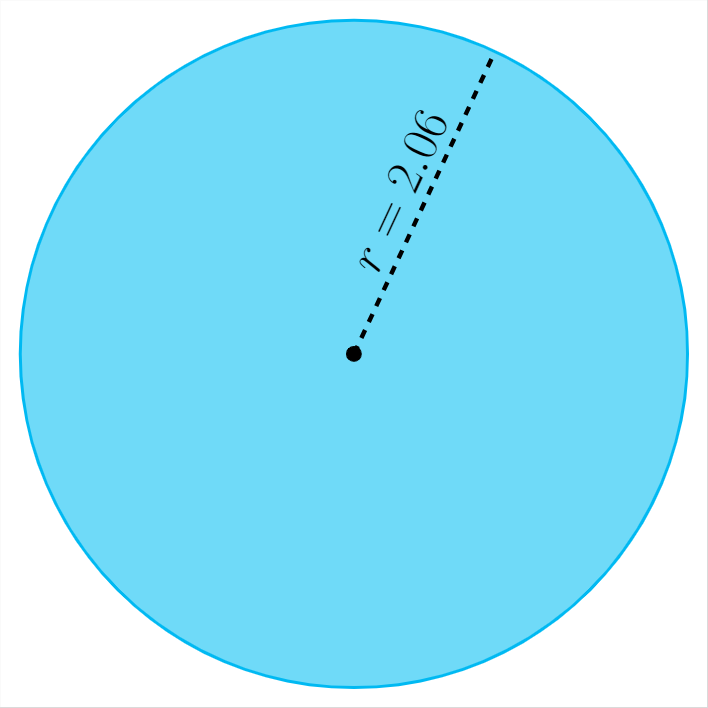
\includegraphics[width=0.85\linewidth]{mex_0001.png}\\
				% Perímetro: \fillin[][0.3in] \quad Área: \fillin[][0.3in]
				\part 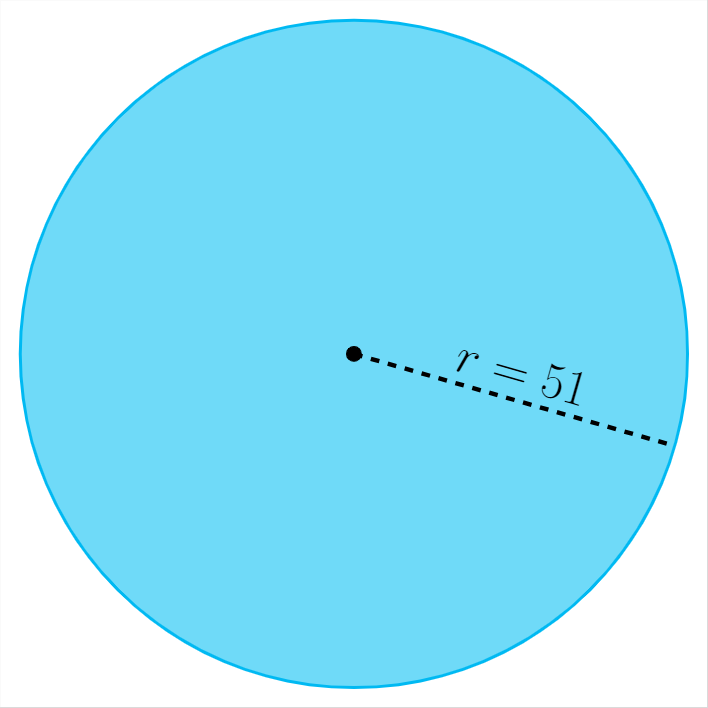
\includegraphics[width=0.85\linewidth]{mex_0002.png}\\

				Perímetro: \\
				\fillin[$P=2\pi r=2(3.14)51=320.28$][0in] \\
				Área: \\
				\fillin[$A=\pi r^2=3.14(51)^2=8167.14$][0in] 

				% \part 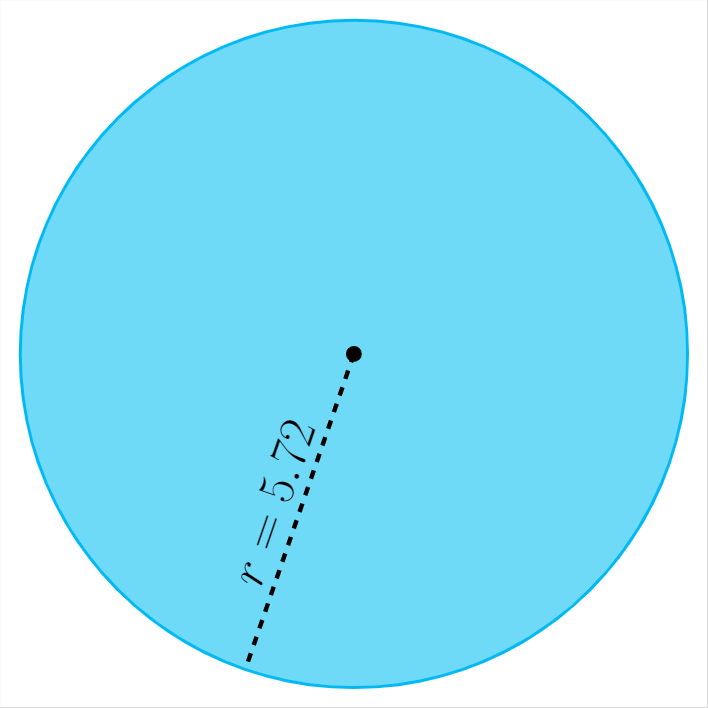
\includegraphics[width=0.85\linewidth]{mex_0003.png}\\
				% Perímetro: \fillin[][0.3in] \quad Área: \fillin[][0.3in]
				% \part 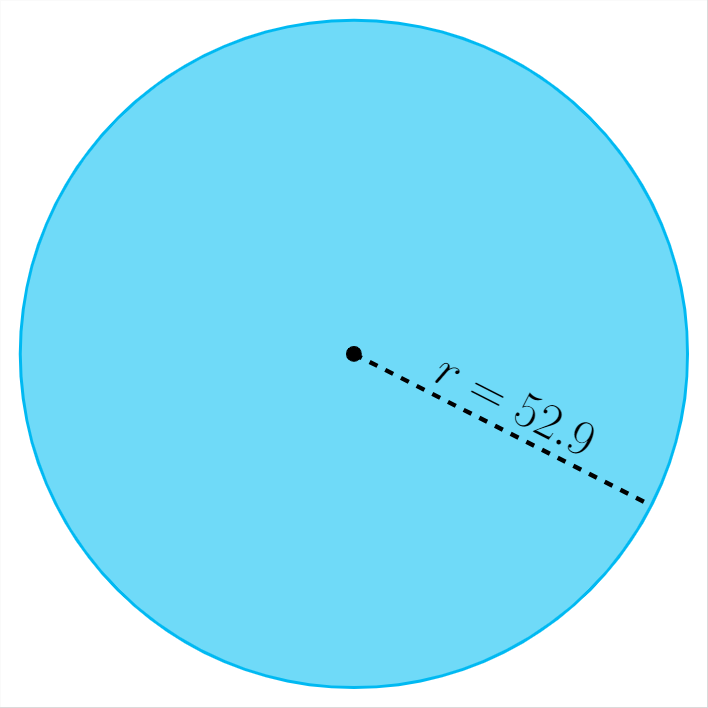
\includegraphics[width=0.85\linewidth]{mex_0004.png}\\
				% Perímetro: \fillin[][0.3in] \quad Área: \fillin[][0.3in]
				\part 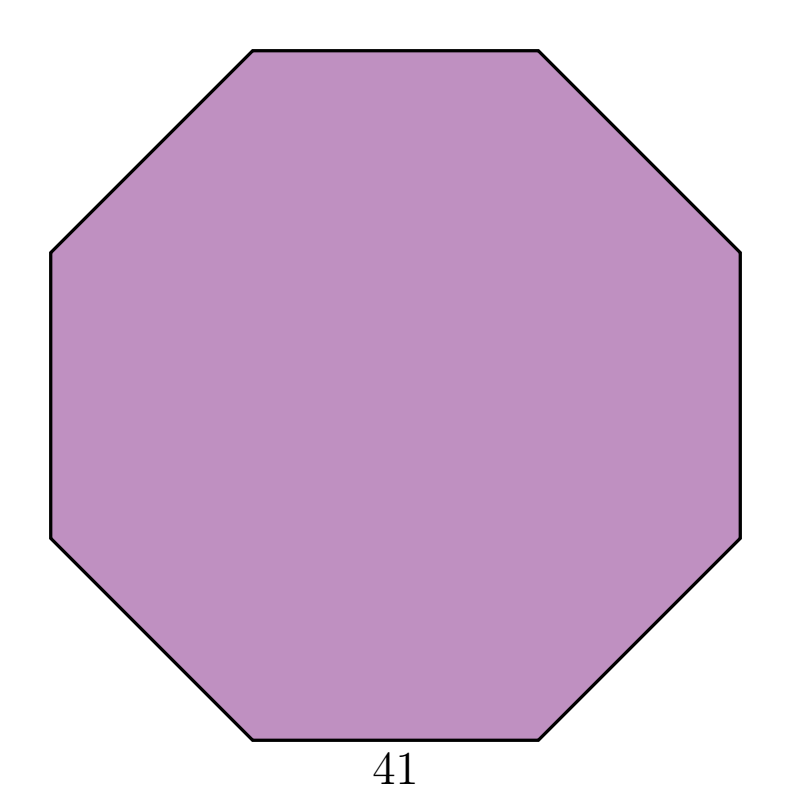
\includegraphics[width=0.85\linewidth]{mex_0005.png}\\

				Perímetro: \\
				\fillin[$P=\pi d=(3.14)14.2=44.58$][0in] \\
				Área: \\
				\fillin[$A=\pi \left(\frac{d}{2}\right)^2=3.14\left(\frac{14.2}{2}\right)^2=158.28$][0in] 

				\part 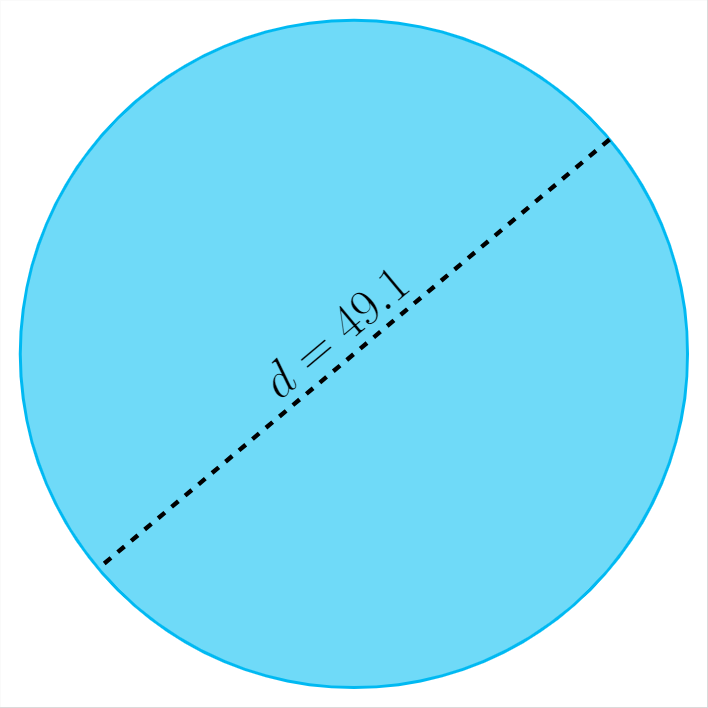
\includegraphics[width=0.85\linewidth]{mex_0009.png}\\

				Perímetro: \\
				\fillin[$P=\pi d=(3.14)49.1=154.17$][0in] \\
				Área: \\
				\fillin[$A=\pi \left(\frac{d}{2}\right)^2=3.14\left(\frac{49.1}{2}\right)^2=1892.48$][0in] 
			\end{parts}
		\end{multicols}
	}

	\questionboxed[3]{Encuentra el \textbf{perímetro} y el \textbf{área} de los siguientes círculos:

		\begin{multicols}{3}
			\begin{parts}
				\part 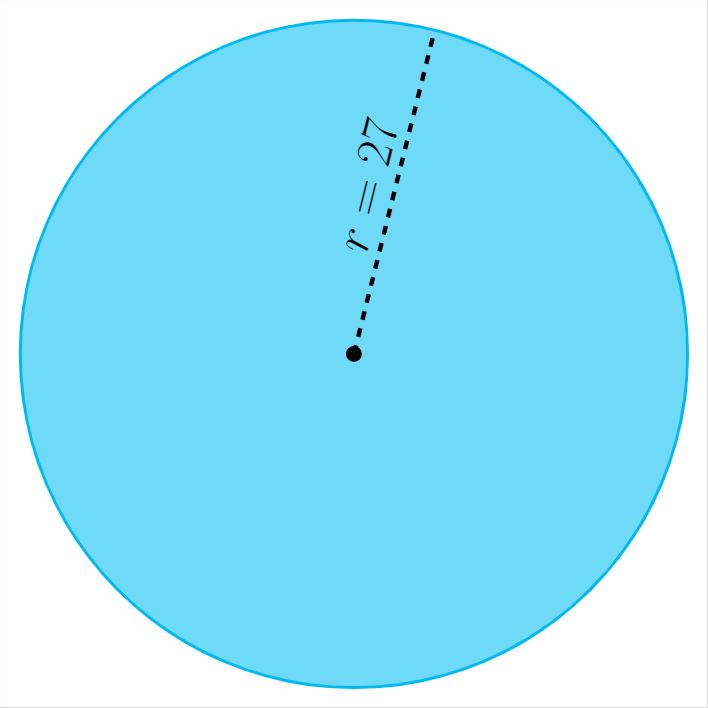
\includegraphics[width=0.85\linewidth]{mex_0006.png}\\

				Perímetro: \\
				\fillin[$P=2\pi r=2(3.14)27=169.56$][0in] \\
				Área: \\
				\fillin[$A=\pi r^2=3.14(27)^2=2289.06$][0in] 

				% \part 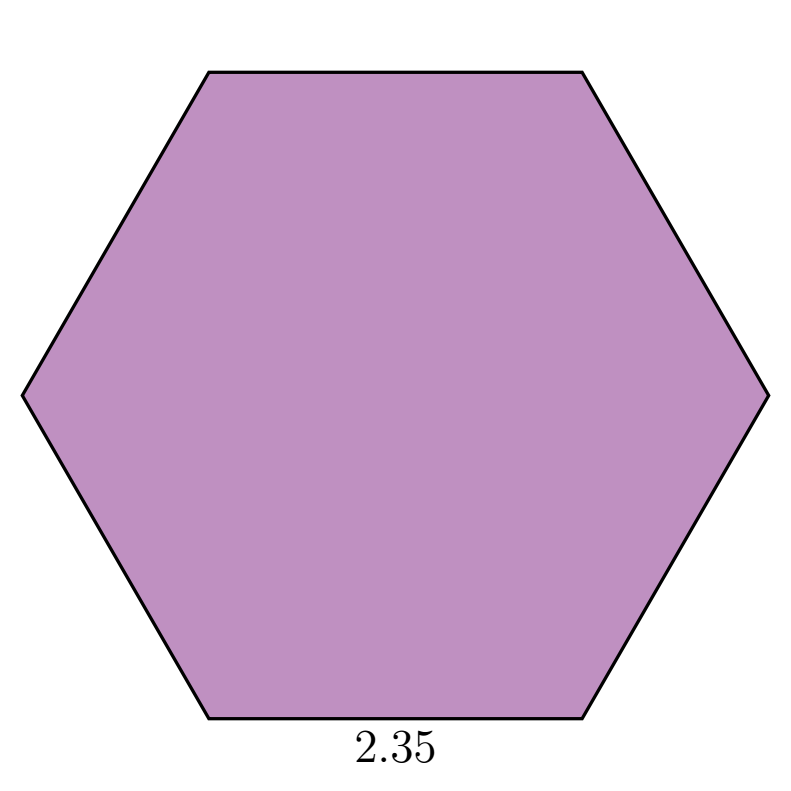
\includegraphics[width=0.85\linewidth]{mex_0007.png}\\
				% Perímetro: \fillin[][0.3in] \quad Área: \fillin[][0.3in]
				\part 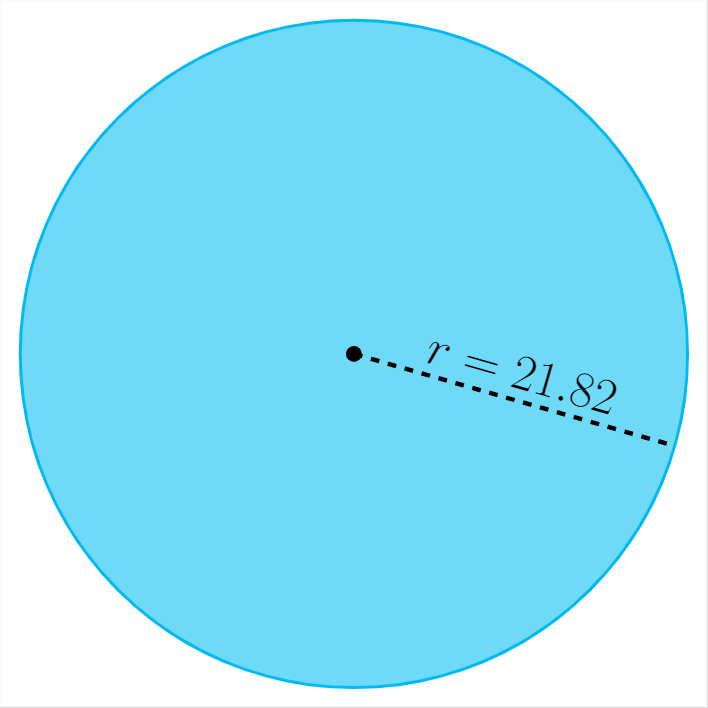
\includegraphics[width=0.85\linewidth]{mex_0008.png}\\

				Perímetro: \\
				\fillin[$P=2\pi r=2(3.14)21.82=137.02$][0in] \\
				Área: \\
				\fillin[$A=\pi r^2=3.14(21.82)^2=1494.99$][0in] 

				% \part 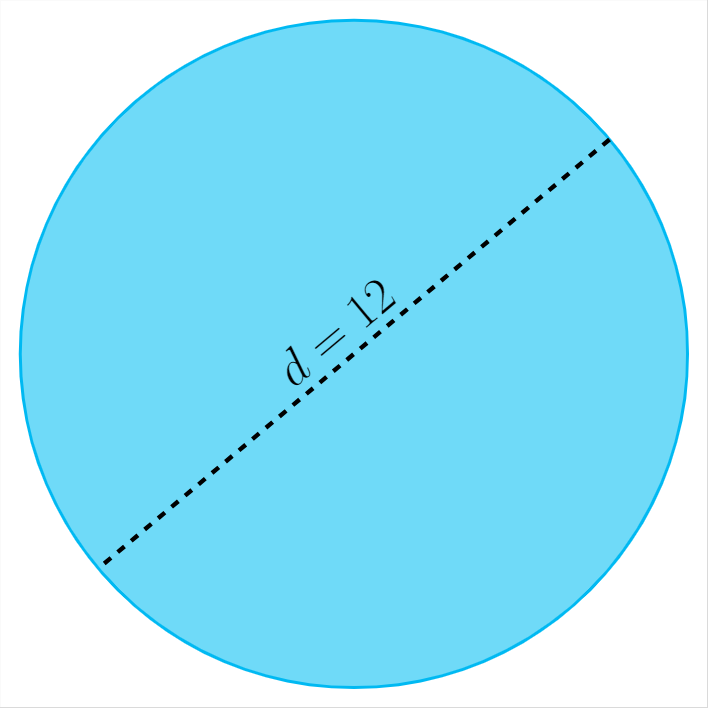
\includegraphics[width=0.85\linewidth]{mex_0010.png}\\
				% Perímetro: \fillin[][0.3in] \quad Área: \fillin[][0.3in]
				\part 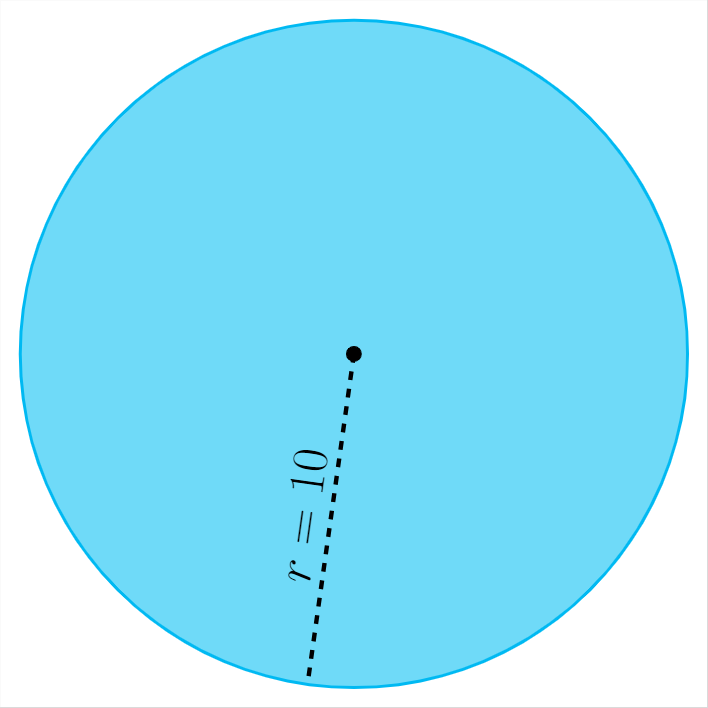
\includegraphics[width=0.85\linewidth]{mex_0011.png}\\

				Perímetro: \\
				\fillin[$P=2\pi r=2(3.14)10=62.8$][0in] \\
				Área: \\
				\fillin[$A=\pi r^2=3.14(10)^2=314$][0in] 

				% \part 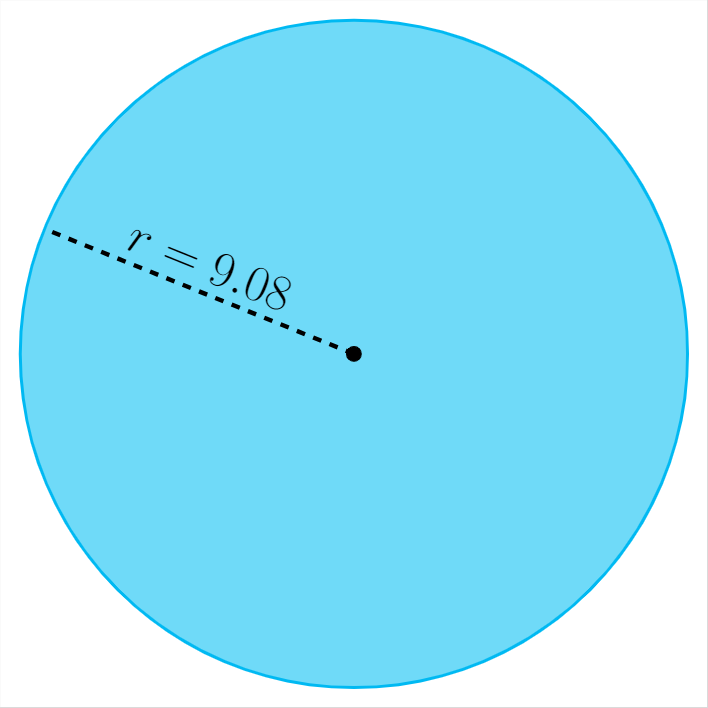
\includegraphics[width=0.85\linewidth]{mex_0012.png}\\
				% Perímetro: \fillin[][0.3in] \quad Área: \fillin[][0.3in]
			\end{parts}
		\end{multicols}
	}

	\newpage
	\section{Polígonos y circunferencias}
	\subsection{Ángulos interiores}

	\questionboxed[4]{Responde a las siguientes preguntas:

		\begin{multicols}{2}
			\begin{parts}
				% \part ¿Cuánto mide el ángulo interior de un hexágono regular? \fillin[$120$][0in]

				% \begin{solutionbox}{2cm}
				% \end{solutionbox}

				% \part ¿Cuánto mide el ángulo interior de un pentadecágono regular? \fillin[$156$][0in]

				% \begin{solutionbox}{2cm}
				% \end{solutionbox}

				\part La suma de los ángulos interiores de un polígono de 8 lados es:% \fillin[$1080$][0in]

				\begin{solutionbox}{1cm}
					\[\Sigma A_I=(n-2)(180^{\circ})=6(180^{\circ})=1080\]
				\end{solutionbox}

				\part ¿Cuánto mide el ángulo interior de un dodecágono regular?% \fillin[$150$][0in]

				\begin{solutionbox}{1cm}
					$A_I=\frac{(n-2)(180^{\circ})}{n} =\frac{(12-2)(180^{\circ})}{12} =150$
				\end{solutionbox}

				\part La suma de los ángulos interiores de un polígono de 11 lados es: %\fillin[$1620$][0in]

				\begin{solutionbox}{1cm}
					\[ \Sigma A_I=(n-2)(180^{\circ})=9(180^{\circ})=1620\]
				\end{solutionbox}

				\part ¿Cuánto mide el ángulo interior de un icoságono regular? %\fillin[$162$][0in]

				\begin{solutionbox}{1cm}
					$A_I=\frac{(n-2)(180^{\circ})}{n}= \frac{(20-2)(180^{\circ})}{20}=162$
				\end{solutionbox}
			\end{parts}
		\end{multicols}
	}

	\subsection{Ángulos centrales y exteriores}

	\questionboxed[4]{Responde a las siguientes preguntas:

		\begin{multicols}{2}
			\begin{parts}
				\part ¿Cuánto mide el ángulo central de un polígono de 9 lados? %\fillin[$40$][0in]

				\begin{solutionbox}{1.2cm}
					\[A_C=\frac{360^{\circ}}{n}=\frac{360^{\circ}}{9}=40^{\circ}\]
				\end{solutionbox}

				\part ¿Cuánto mide el ángulo exterior de un polígono de 10 lados? %\fillin[$36$][0in]

				\begin{solutionbox}{1.2cm}
					\[A_E=\frac{360^{\circ}}{n}=\frac{360^{\circ}}{10}=36^{\circ}\]
				\end{solutionbox}

				% \part ¿Cuánto mide el ángulo central de un polígono de 15 lados? \fillin[$24$][0in]

				% \begin{solutionbox}{2cm}
				% \end{solutionbox}

				% \part ¿Cuánto mide el ángulo central de un polígono de 12 lados? \fillin[$30$][0in]

				% \begin{solutionbox}{2cm}
				% \end{solutionbox}

				\part ¿Cuánto mide el ángulo exterior de un polígono de 6 lados? %\fillin[$60$][0in]

				\begin{solutionbox}{1.2cm}
					\[A_E=\frac{360^{\circ}}{n}=\frac{360^{\circ}}{6}=60^{\circ}\]
				\end{solutionbox}

				\part ¿Cuánto mide el ángulo central de un polígono de 20 lados? %\fillin[$18$][0in]

				\begin{solutionbox}{1.2cm}
					\[A_C=\frac{360^{\circ}}{n}=\frac{360^{\circ}}{20}=18^{\circ}\]
				\end{solutionbox}

			\end{parts}
		\end{multicols}
	}

	\subsection{Ángulos centrales e inscritos}

	\questionboxed[6]{Calcula el valor del \textbf{ángulo} $x$:

		\begin{multicols}{3}
			\begin{parts}
				\part 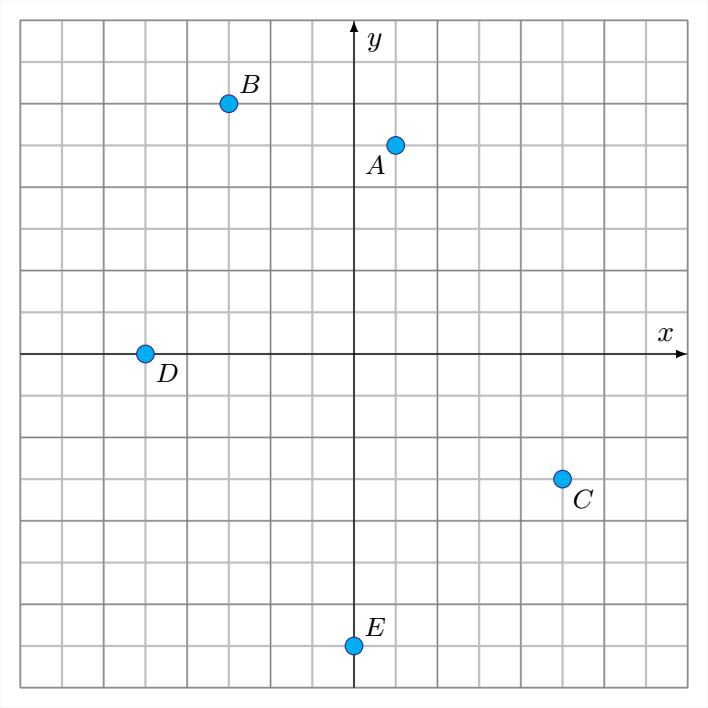
\includegraphics[width=.7\linewidth]{mex_0043.png}
				$x=$\fillin[$136^{\circ}$][0in]

				\part 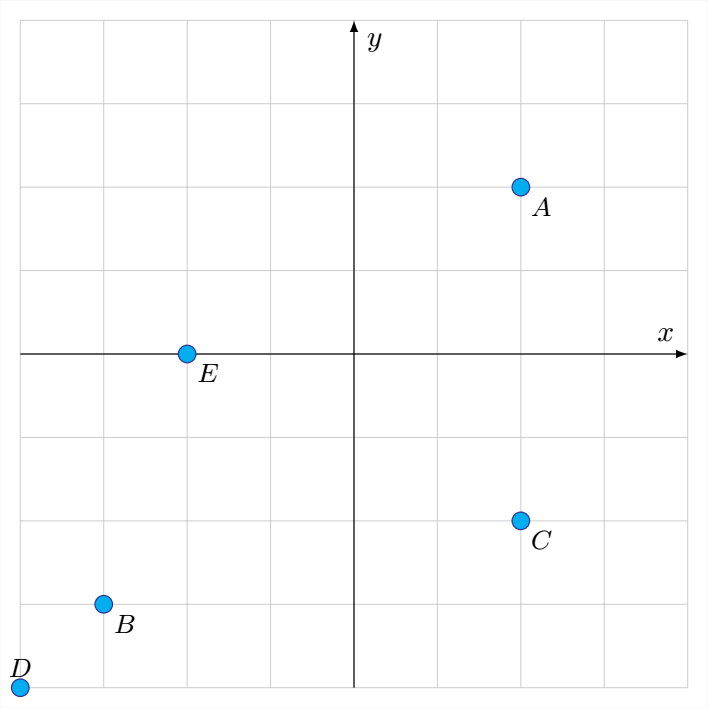
\includegraphics[width=.7\linewidth]{mex_0044.png}
				$x=$\fillin[$80^{\circ}$][0in]

				\part 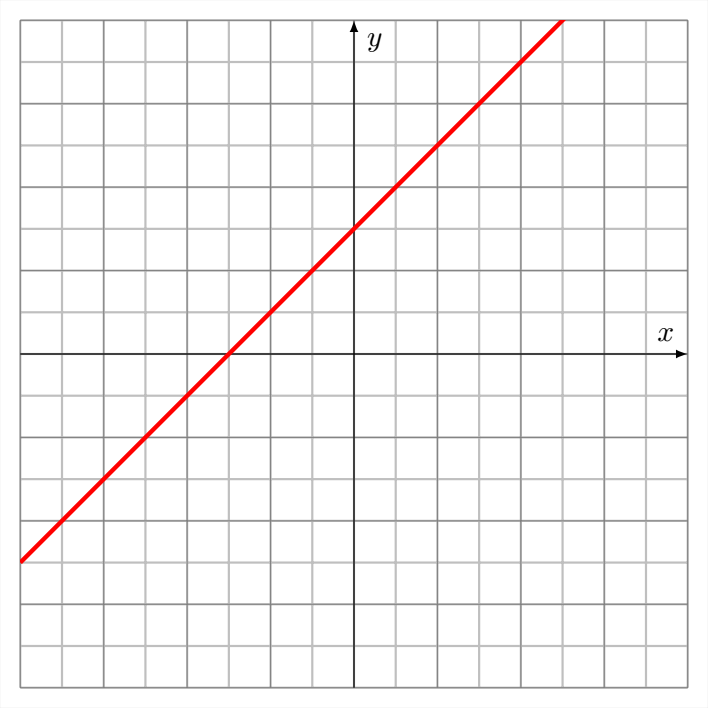
\includegraphics[width=.7\linewidth]{mex_0046.png}
				$x=$\fillin[$156^{\circ}$][0in]

				\part 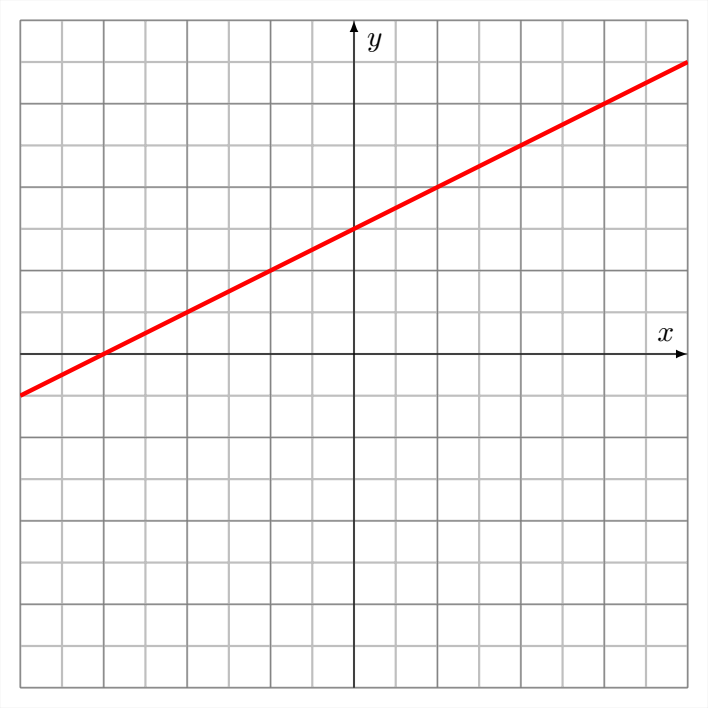
\includegraphics[width=.7\linewidth]{mex_0047.png}
				$x=$\fillin[$56^{\circ}$][0in]

				\part 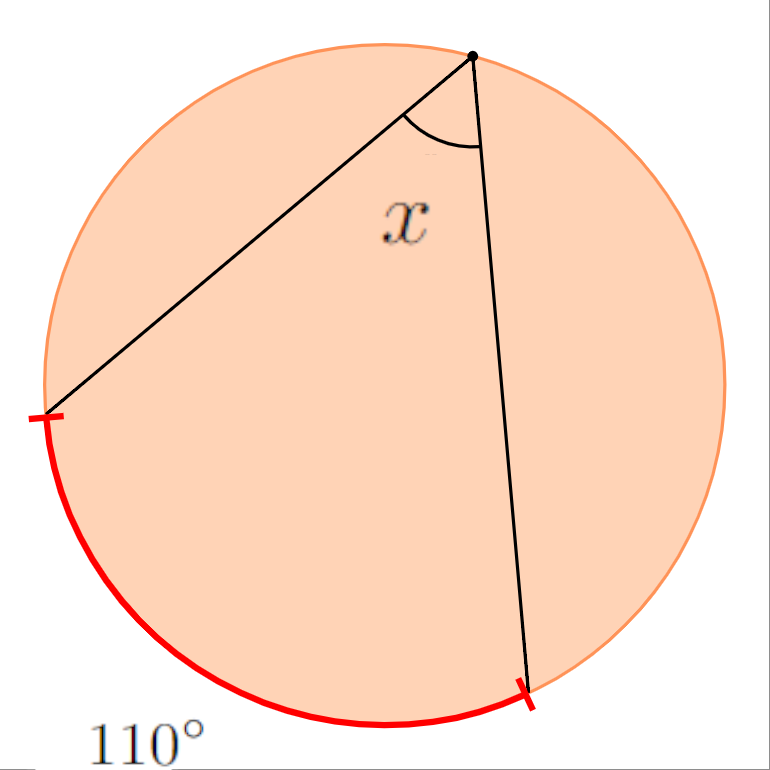
\includegraphics[width=.7\linewidth]{mex_0049.png}
				$x=$\fillin[$55^{\circ}$][0in]

				\part 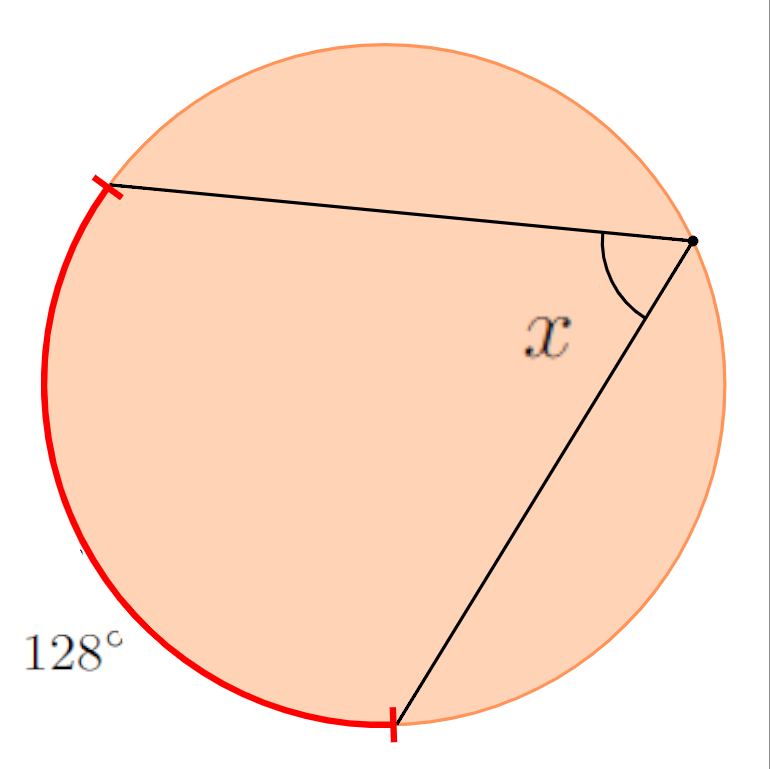
\includegraphics[width=.7\linewidth]{mex_0050.png}
				$x=$\fillin[$64^{\circ}$][0in]
			\end{parts}
		\end{multicols}
	}

	\subsection{Arco de una circunferencia}

	\questionboxed[6]{Calcula el valor del \textbf{arco} $x$:

		\begin{multicols}{3}
			\begin{parts}
				\part 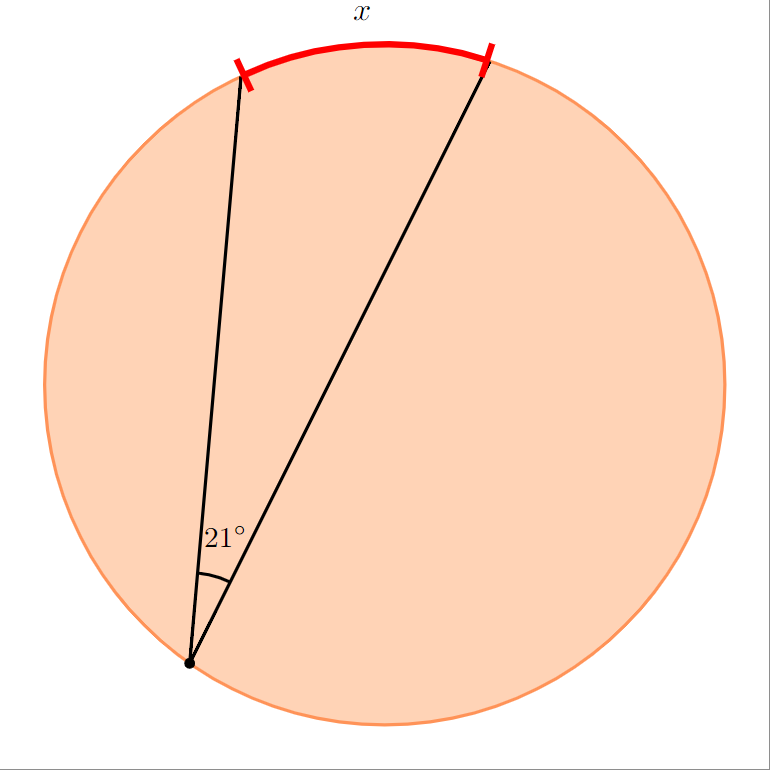
\includegraphics[width=.7\linewidth]{mex_0052.png}
				$x=$\fillin[$42$][0in]

				\part 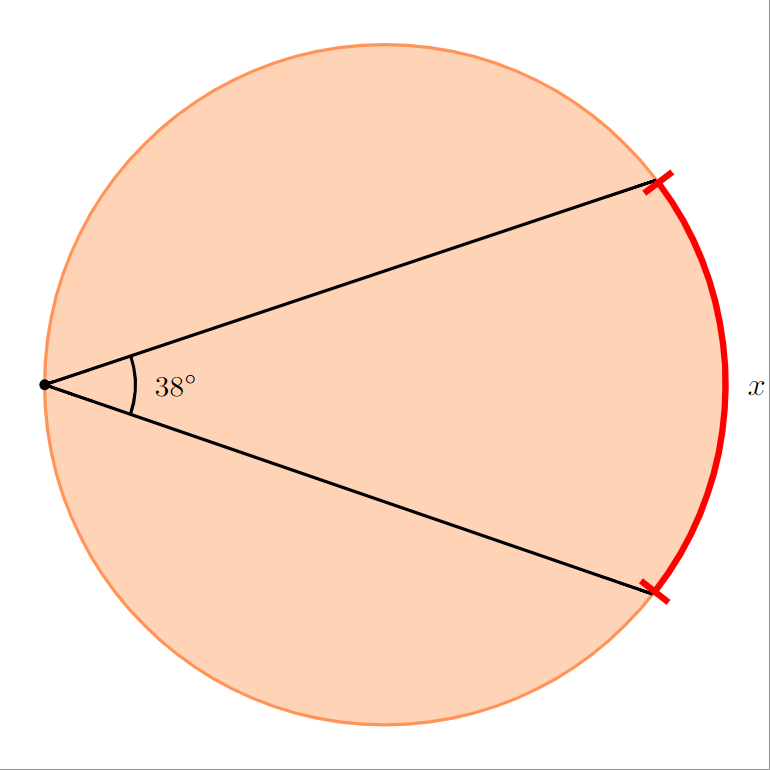
\includegraphics[width=.7\linewidth]{mex_0053.png}
				$x=$\fillin[$76$][0in]

				\part 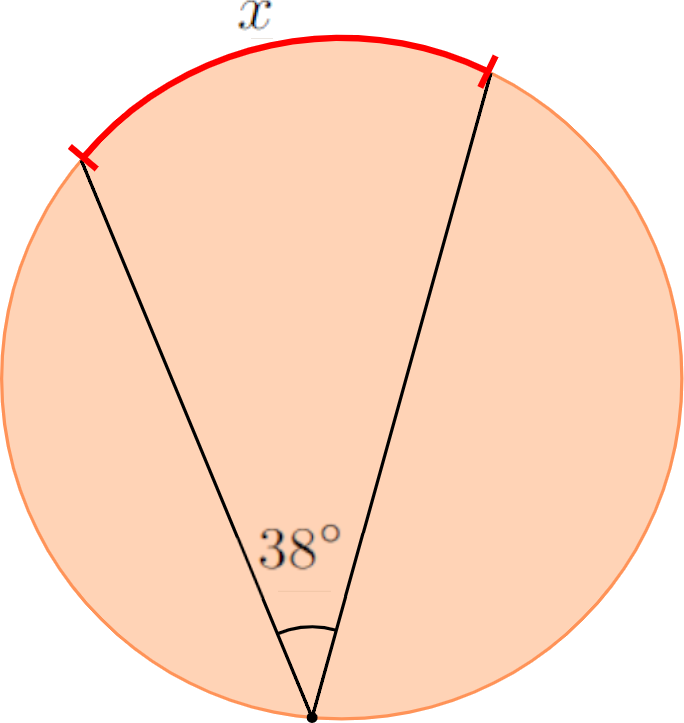
\includegraphics[width=.7\linewidth]{mex_0054.png}
				$x=$\fillin[$76$][0in]

				\part 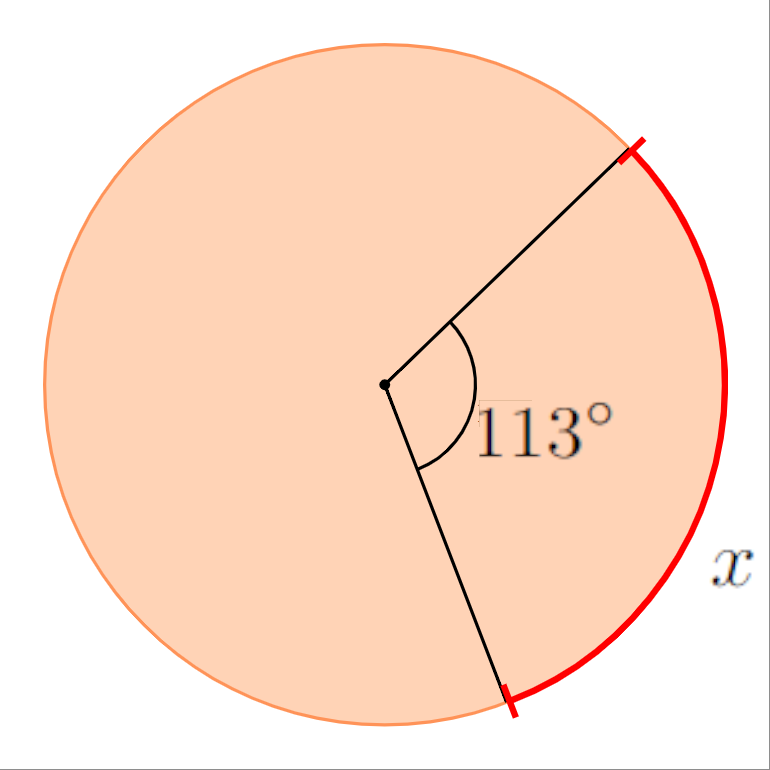
\includegraphics[width=.7\linewidth]{mex_0055.png}
				$x=$\fillin[$113$][0in]

				\part 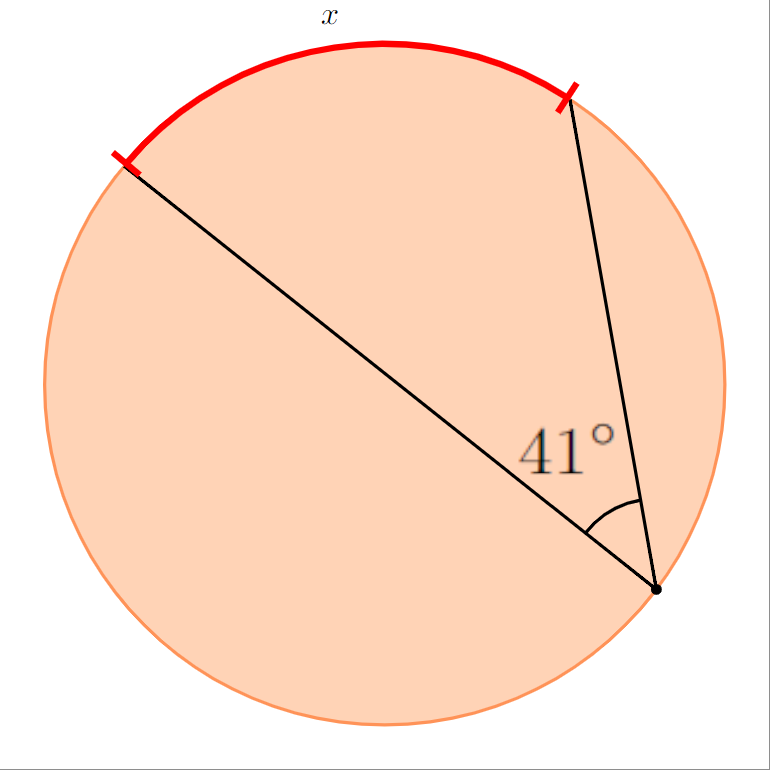
\includegraphics[width=.7\linewidth]{mex_0056.png}
				$x=$\fillin[$82$][0in]

				\part 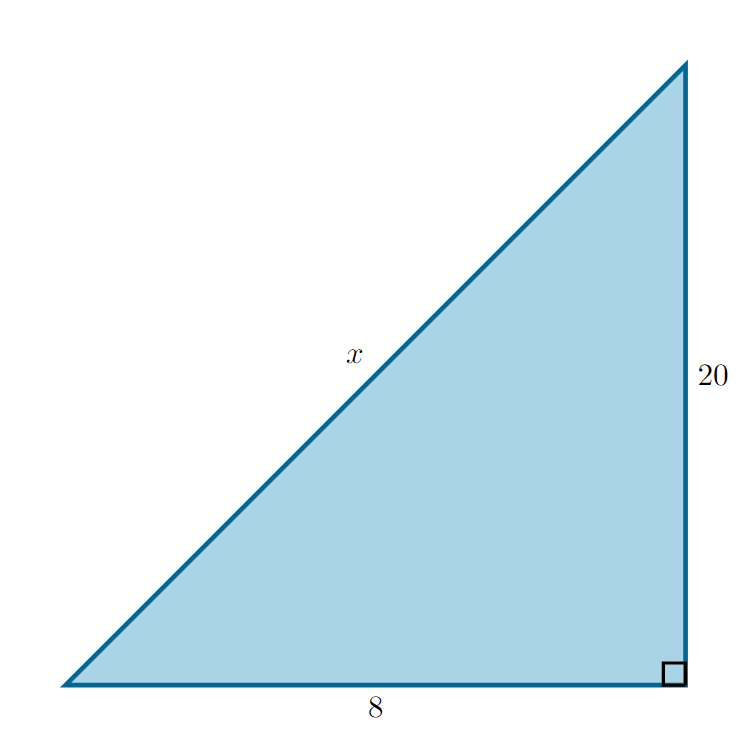
\includegraphics[width=.7\linewidth]{mex_0057.png}
				$x=$\fillin[$83$][0in]
			\end{parts}
		\end{multicols}
	}

	\subsection{Área de un sector circular}

	\questionboxed[6]{Calcula el \textbf{área} de cada uno de los siguientes sectores circulares:

		\begin{multicols}{3}
			\begin{parts}
				\part 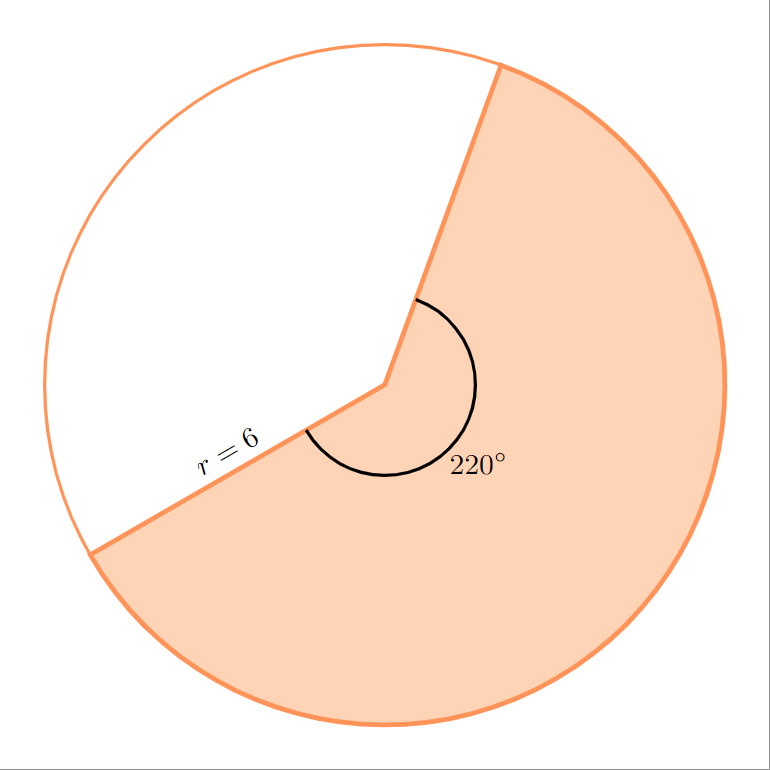
\includegraphics[width=.7\linewidth]{mex_0058.png}

				\begin{solutionbox}{2cm}
					\[ A=\pi r^2\left(\frac{x}{360}\right)\]
					$A=3.14(6)^2\left(\frac{220}{360}\right)=69.08$
				\end{solutionbox}

				\part 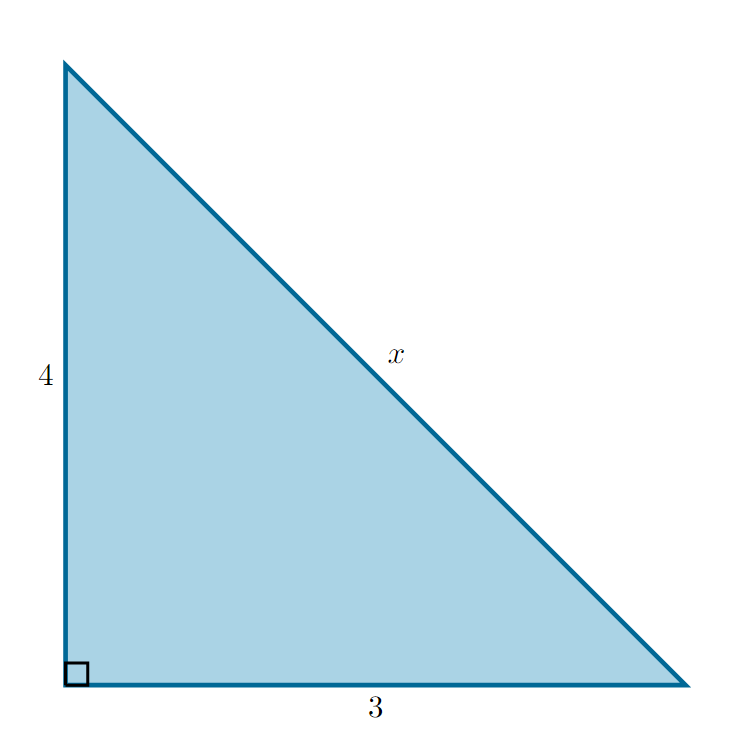
\includegraphics[width=.7\linewidth]{mex_0059.png}

				\begin{solutionbox}{2cm}
					\[ A=\pi r^2\left(\frac{x}{360}\right)\]
					$A=3.14(2)^2\left(\frac{104}{360}\right)=3.62$
				\end{solutionbox}

				\part 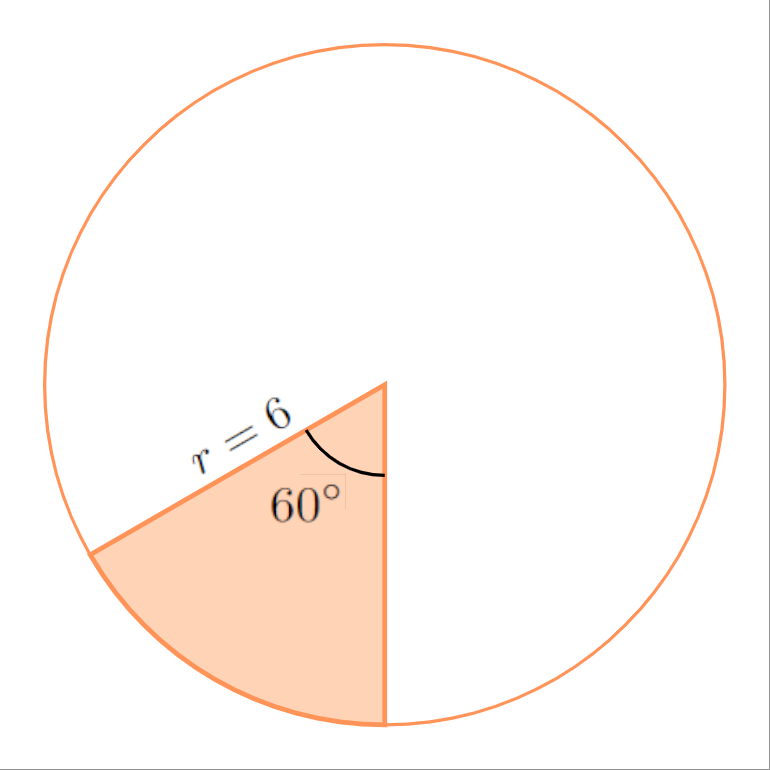
\includegraphics[width=.7\linewidth]{mex_0060.png}

				\begin{solutionbox}{2cm}
					\[ A=\pi r^2\left(\frac{x}{360}\right)\]
					$A=3.14(6)^2\left(\frac{60}{360}\right)=18.84$
				\end{solutionbox}

				\part 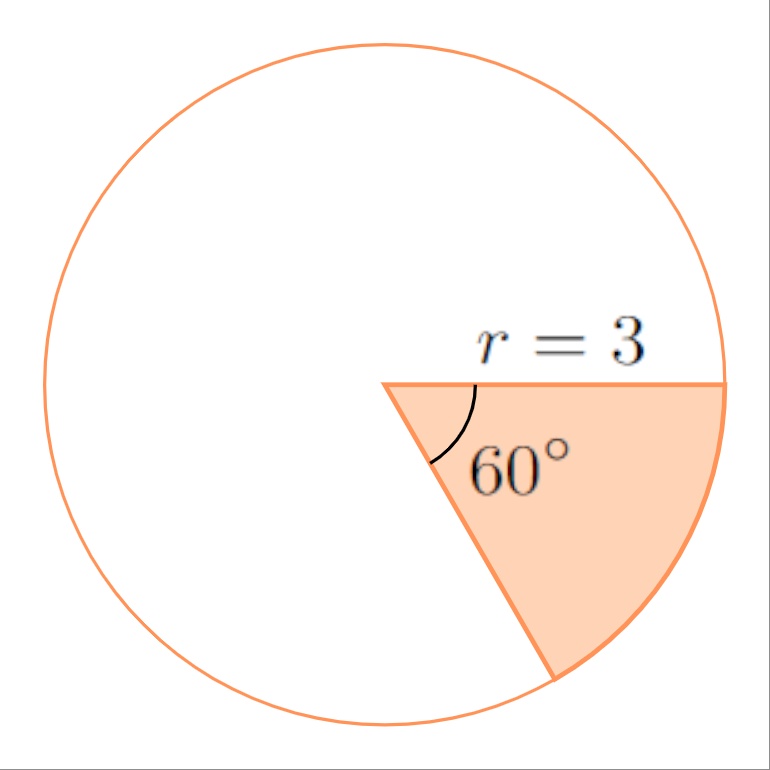
\includegraphics[width=.7\linewidth]{mex_0061.png}

				\begin{solutionbox}{2cm}
					\[ A=\pi r^2\left(\frac{x}{360}\right)\]
					$A=3.14(3)^2\left(\frac{60}{360}\right)=4.71$
				\end{solutionbox}

				\part 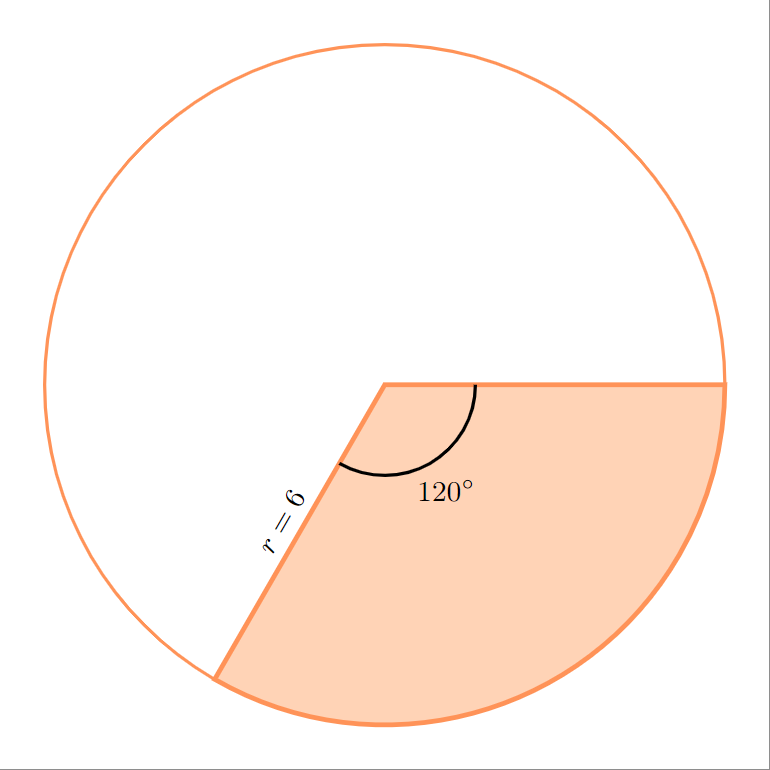
\includegraphics[width=.7\linewidth]{mex_0062.png}

				\begin{solutionbox}{2cm}
					\[ A=\pi r^2\left(\frac{x}{360}\right)\]
					$A=3.14(6)^2\left(\frac{120}{360}\right)=37.68$
				\end{solutionbox}

				\part 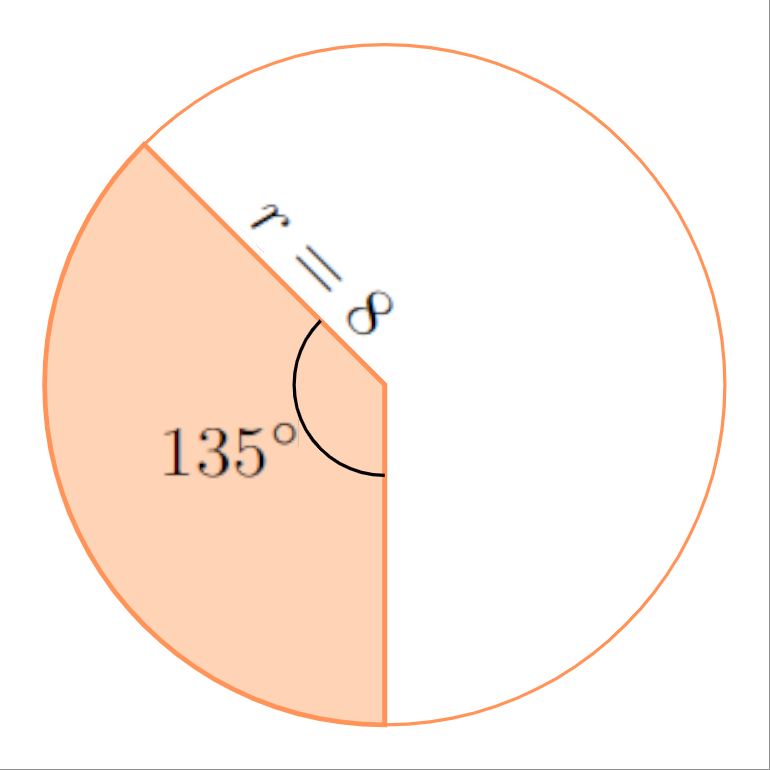
\includegraphics[width=.7\linewidth]{mex_0063.png}

				\begin{solutionbox}{2cm}
					\[ A=\pi r^2\left(\frac{x}{360}\right)\]
					$A=3.14(8)^2\left(\frac{135}{360}\right)=75.36$
				\end{solutionbox}

			\end{parts}
		\end{multicols}
	}

	\section{Figuras y cuerpos geométricos}

	\subsection{Perímetro y Área}

	\questionboxed[2]{Encuentra el \textbf{perímetro} y el \textbf{área} de las siguientes figuras:

		\begin{multicols}{3}
			\begin{parts}\footnotesize%
				% \part 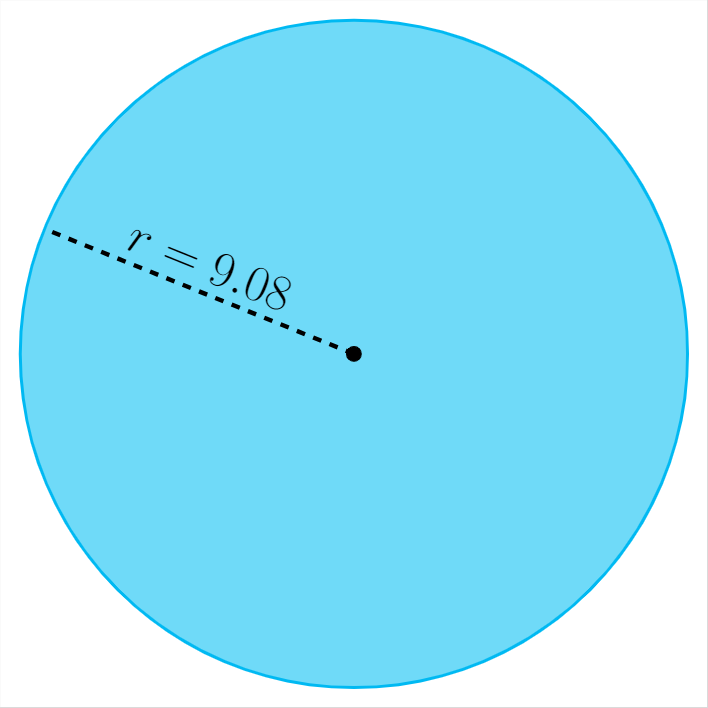
\includegraphics[width=\linewidth]{mex_0013.png}
				% Perímetro: \\
				% \fillin[$P=(12\times 3) + (8\times 2)=36+16=52$][0in] \\
				% Área: \\
				% \fillin[$A=12^2+\dfrac{8^2}{2}=144+32=177$][0in]

				\part 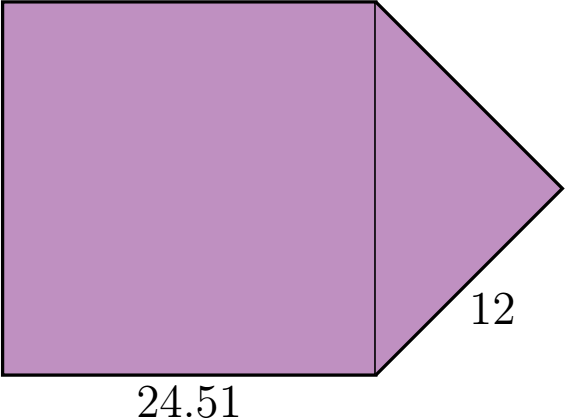
\includegraphics[width=.7\linewidth]{mex_0014.png} 

				Perímetro: \\
				\fillin[$P=(3)24.51 + (2)12= 73.53+24=97.53$][0in] 

				Área: \\
				\fillin[$A=24.51^2+\dfrac{12^2}{2}=600.74+72=672.74$][0in]

				% \part 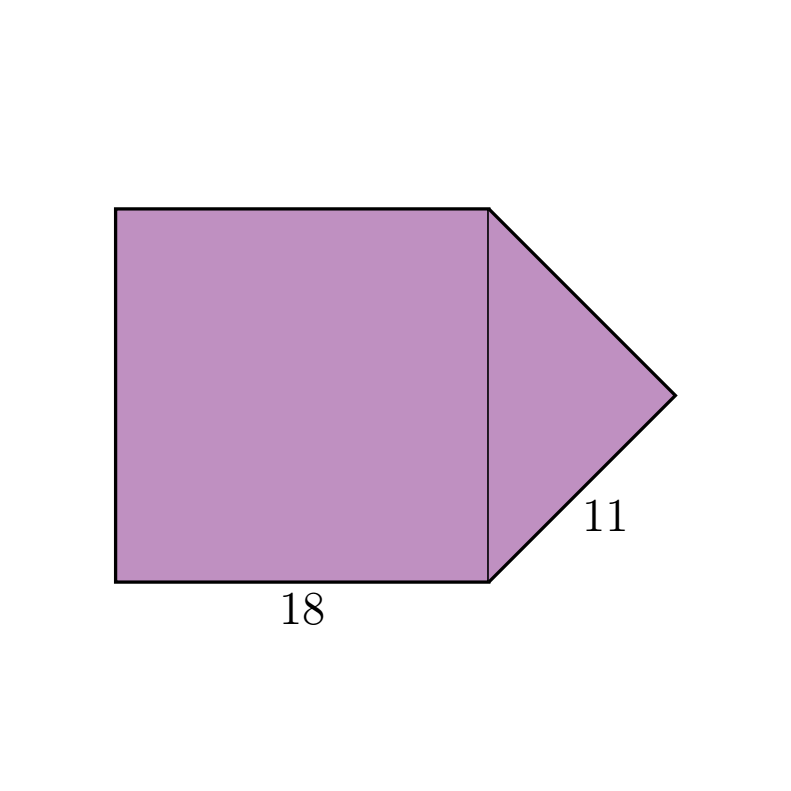
\includegraphics[width=.5\linewidth]{mex_0015.png}
				% Perímetro: \\
				% \fillin[$P=(18\times 3) + (11\times 2)=36+16=52$][0in] \\
				% Área: \\
				% \fillin[$A=18^2+\dfrac{11^2}{2}=324+60.5=384.5$][0in]

				% \part 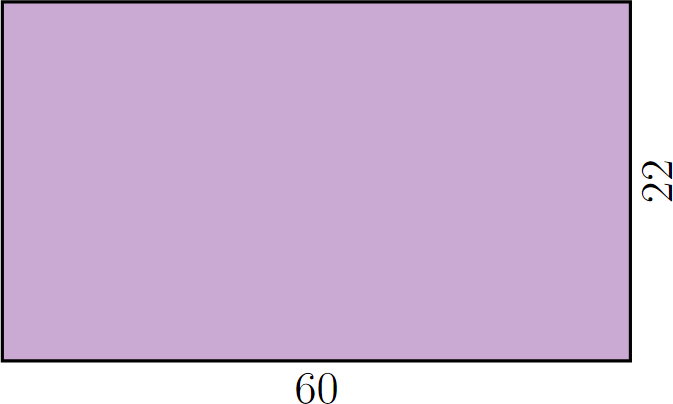
\includegraphics[width=\linewidth]{mex_0019.png}
				% Perímetro: \\
				% \fillin[$P=(60\times 2) + (22\times 2)=120+44=164$][0in] \\
				% Área: \\
				% \fillin[$A=60\times 22=1320$][0in]

				\part 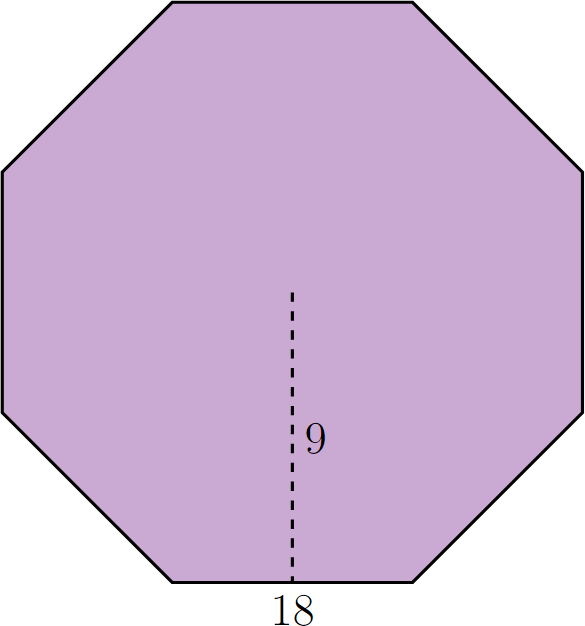
\includegraphics[width=.5\linewidth]{mex_0016.png} 

				Perímetro: \\
				\fillin[$P=18\times 8 =144$][0in] 

				Área: \\
				\fillin[$A=\dfrac{8\times 18 \times 9}{2}=648$][0in]

				\part 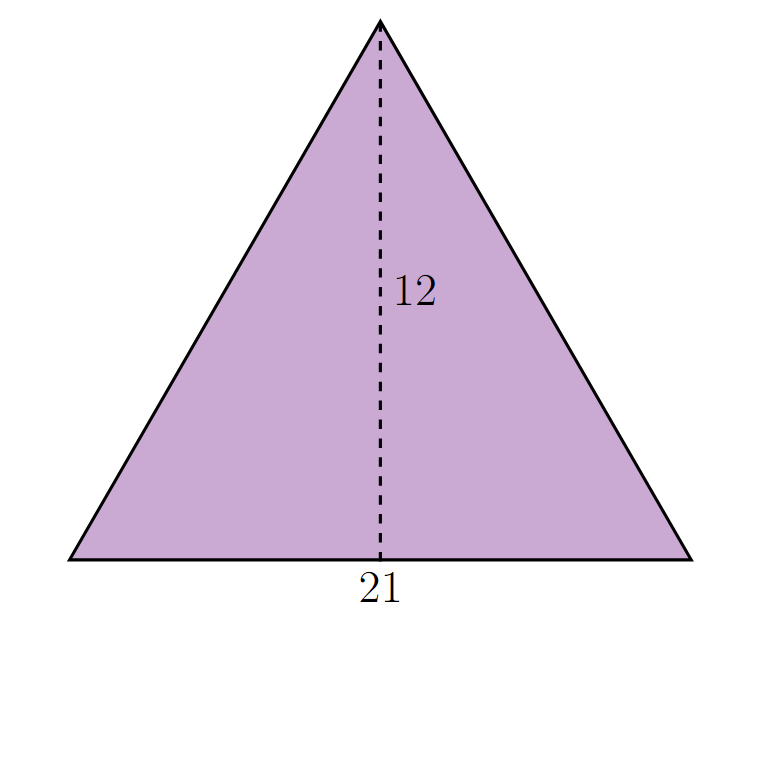
\includegraphics[width=.8\linewidth]{mex_0020.png} 

				Perímetro: \\
				\fillin[$P=(2)61+(2)29=122+58=180$][0in] 

				Área: \\
				\fillin[$A=61\times 29=1769$][0in]

				

				%  \part 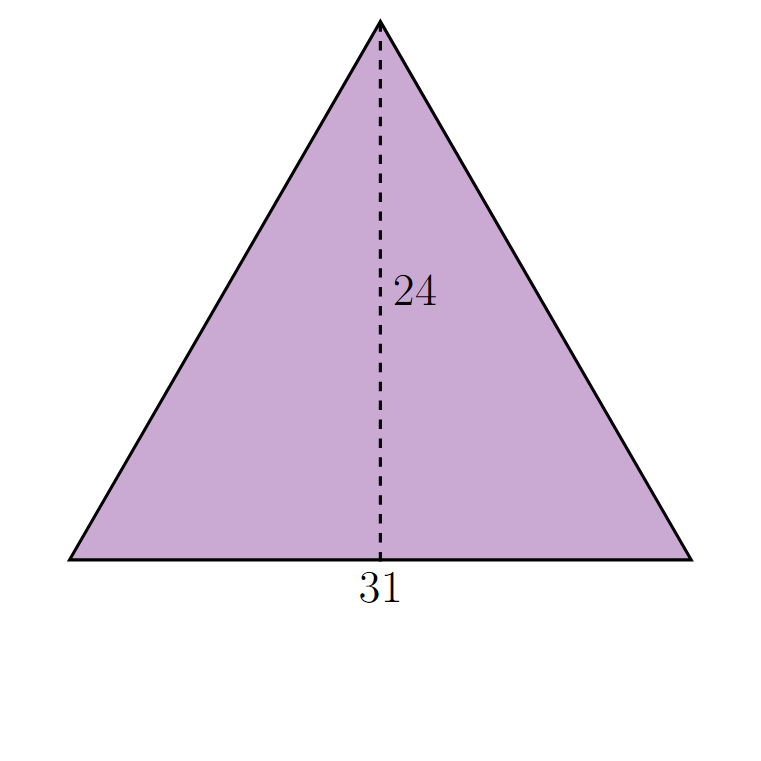
\includegraphics[width=.5\linewidth]{mex_0017.png}
				%  Perímetro: \\
				%  \fillin[$P=(31\times 3) =93$][0in] \\
				%  Área: \\
				%  \fillin[$A=\frac{31\times 24}{2}=372$][0in]

				%  \part 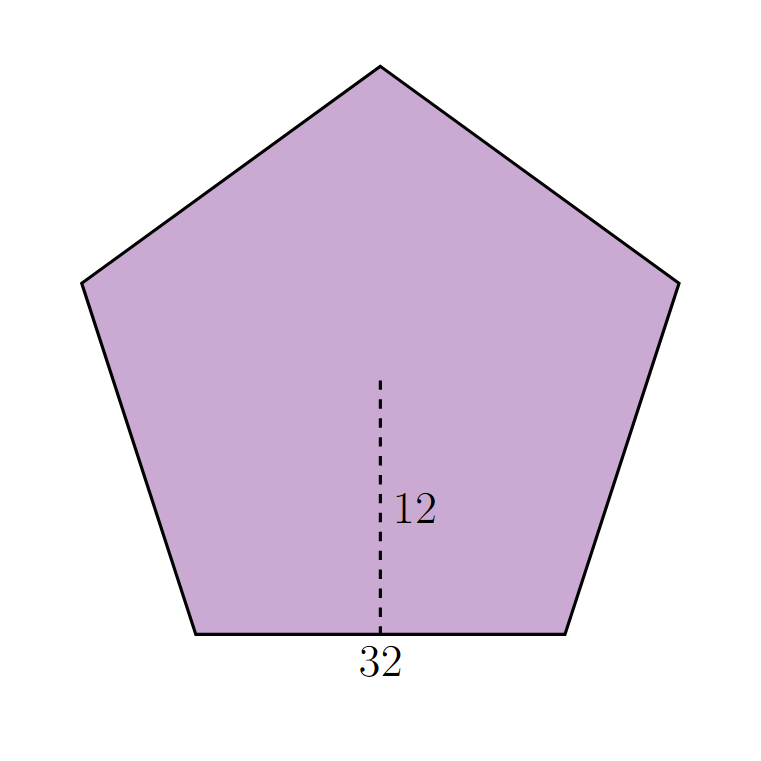
\includegraphics[width=.5\linewidth]{mex_0018.png}
				%  Perímetro: \\
				% \fillin[$P=32\times 5 =160$][0in] \\
				% Área: \\
				% \fillin[$A=\dfrac{5\times 32 \times 12}{2}=960$][0in]
			\end{parts}
		\end{multicols}
	}

	\subsection{Resolución de problemas}

	\questionboxed[4]{Resuelve los siguientes problemas:

		\begin{multicols}{2}
			\begin{parts}\footnotesize%
				\part Calcula la altura de un prisma que tiene como área de la base 6 m$^2$ y 99 m$^3$ de capacidad.

				\begin{solutionbox}{2cm}
					Ya que el volumen de un prisma es: $V=A_b\cdot h$, entonces la altura del prisma es: \[h=\dfrac{V}{A_b}=\dfrac{99}{6}=16.5\text{m}\]
				\end{solutionbox}

				\part ¿Cuál es el perímetro de un campo de fútbol que mide 95.12 metros de largo y 45.27 metros de ancho?

				\begin{solutionbox}{1.8cm}
					El perímetro de un rectángulo es: $P=2(l+a)$ entonces el perímetro del campo de fútbol es: \[P=2(95.12+45.27)=280.78\text{m}\]
				\end{solutionbox}

				\columnbreak%

				\part Calcula la altura de un prisma que tiene como área de la base 8 m$^2$ y 144 m$^3$ de capacidad.

				\begin{solutionbox}{2cm}
					Ya que el volumen de un prisma es: $V=A_b\cdot h$, entonces la altura del prisma es: \[h=\dfrac{V}{A_b}=\dfrac{144}{8}=18\text{m}\].
				\end{solutionbox}				

				\part Ricardo quiere poner una barda alrededor de un terreno pentagonal que mide 15 metros por lado. ¿Cuánta barda necesitará Ricardo para poner barda en todo el terreno?

				\begin{solutionbox}{1.8cm}
					Se sabe que el perímetro de un pentágono es: $P=5l$, entonces el perímetro del terreno es: \[P=5(15)=75\text{m}\]
				\end{solutionbox}
			\end{parts}
		\end{multicols}
	}

	\subsection{Área lateral, Área total y Volumen}


	\questionboxed[2]{Calcula el \textbf{volumen}, el \textbf{área lateral} y el \textbf{área total} de las siguientes figuras:

			\begin{parts}
				\part Cilindro con altura $h=17$ cm y un radio $r=4$ cm.

				\begin{minipage}{.25\linewidth}
					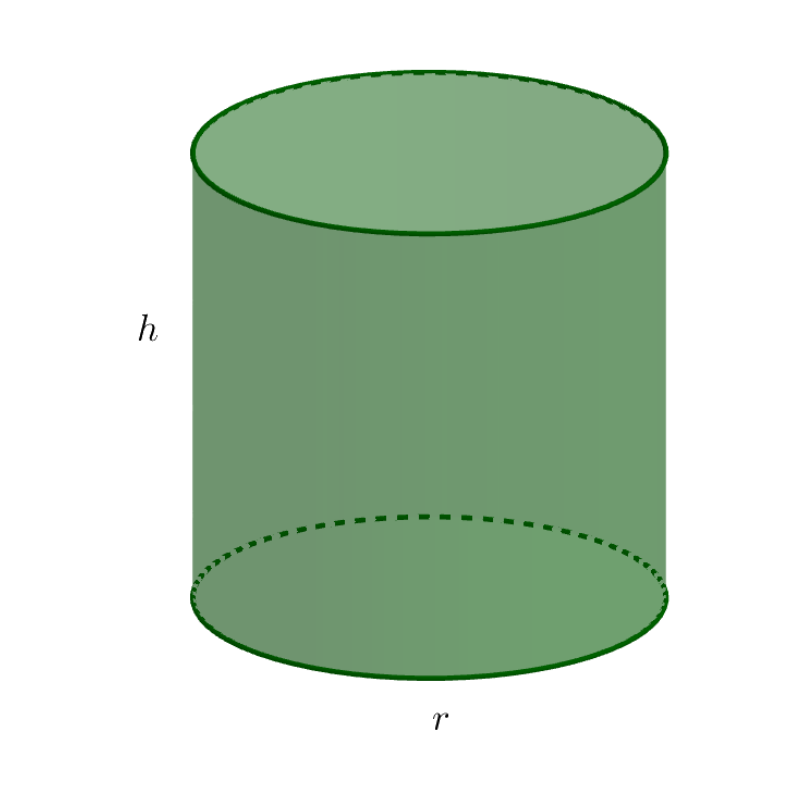
\includegraphics[width=0.8\linewidth]{mex_0024.png}
				\end{minipage}\hfill
				\begin{minipage}{.75\linewidth}
					Volumen:\\[-2em]
					\begin{solutionbox}{1cm}
						\[V=\pi r^2h=(3.14) 4^2\cdot 17= 857.12\]
					\end{solutionbox}
					
					A. Lateral:\\[-2em]
					\begin{solutionbox}{1cm}
						\[A_L=2\pi rh=2(3.14) 4\cdot 17= 2(3.14) 68=428.48\]
					\end{solutionbox}
					
					A. Total:\\[-2em]
					\begin{solutionbox}{1cm}
						\[A_T=A_L+2\pi r^2=428.48+2(3.14) 16=528.96\]
					\end{solutionbox}
				\end{minipage}

				\part Prisma octagonal de 19 cm de altura y su base es un octágono cuyos lados $l$ miden 7 cm y un apotema $a$ de 5 cm.
				
				\begin{minipage}{.25\linewidth}
					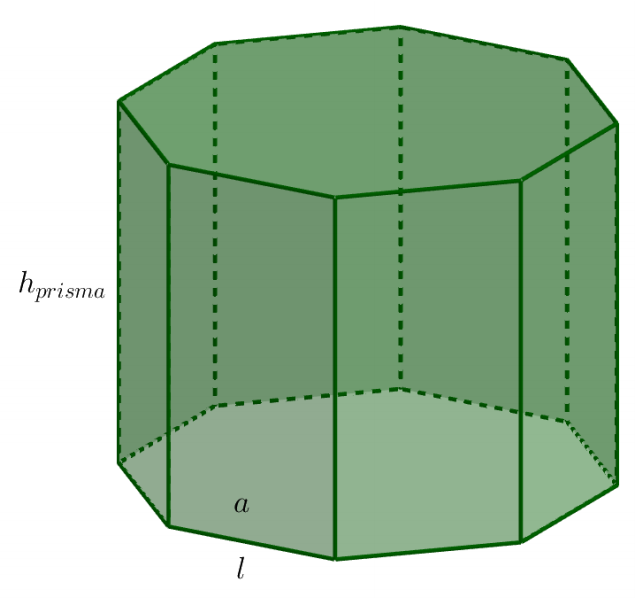
\includegraphics[width=0.8\linewidth]{mex_0025.png}
				\end{minipage}\hfill
				\begin{minipage}{.75\linewidth}
					Volumen:\\[-2em]
					\begin{solutionbox}{1cm}
						\[V=A_b\cdot h= \left(\dfrac{nla}{2}\right)h= \dfrac{8(7)5}{2}(19)=2660\]
					\end{solutionbox}
					
					A. Lateral:\\[-2em]
					\begin{solutionbox}{1cm}
						\[A_L=nlh=8(7)19= 1064\]
					\end{solutionbox}
					
					A. Total:\\[-2em]
					\begin{solutionbox}{1cm}
						\[A_T=A_L+2\dfrac{nla}{2}=A_L+nla=1064+280=1344\]
					\end{solutionbox}
				\end{minipage}
			\end{parts}
	}
	
	\questionboxed[2]{Calcula el \textbf{volumen}, el \textbf{área lateral} y el \textbf{área total} de las siguientes figuras:

		\begin{parts}
			\part Pirámide cuyos lados "l" de la base miden 16 cm y la altura "h" mide 27 cm.

			\begin{minipage}{.25\linewidth}
				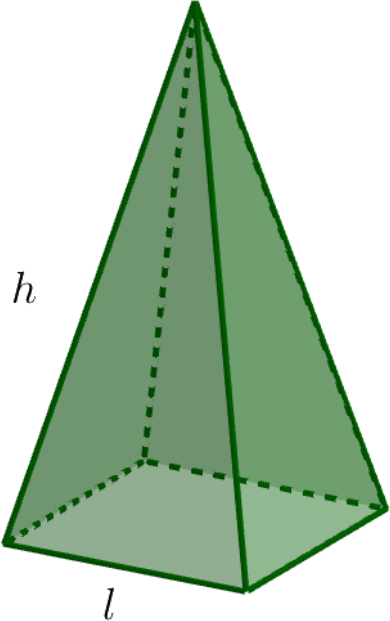
\includegraphics[width=0.6\linewidth]{mex_0029.png}
			\end{minipage}\hfill
			\begin{minipage}{.75\linewidth}
				Volumen:\\[-2em]
				\begin{solutionbox}{1cm}
					\[V=\dfrac{1}{3}A_b h= \dfrac{1}{3}l^2h= \dfrac{1}{3}16^2(27)=2304\]
				\end{solutionbox}

				A. Lateral:\\[-2em]
				\begin{solutionbox}{1cm}
					\[A_L=n\dfrac{lh}{2}=4\cdot \dfrac{16\times 27}{2}=864\]
				\end{solutionbox}

				A. Total:\\[-2em]
				\begin{solutionbox}{1cm}
					\[A_T=A_L+l^2=864+16^2=864+256=1120\]
				\end{solutionbox}
			\end{minipage}

			\part Pirámide de 19 cm de altura cuya base es un pentágono cuyos lados "l" miden 8 cm y su apotema mide 5 cm.

			\begin{minipage}{.25\linewidth}
				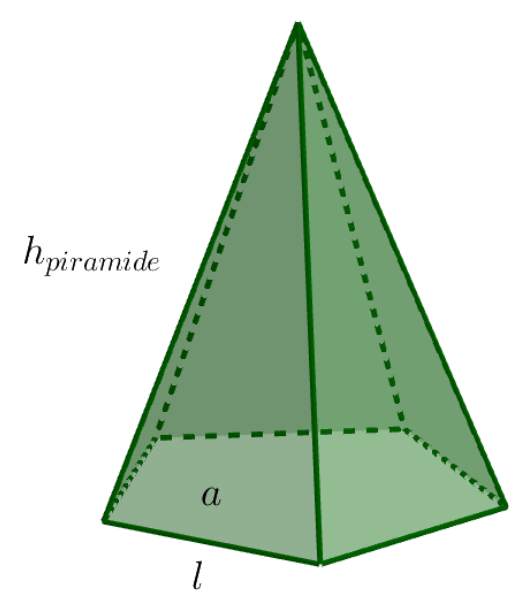
\includegraphics[width=0.8\linewidth]{mex_0027.png}
			\end{minipage}\hfill
			\begin{minipage}{.75\linewidth}
				Volumen:\\[-2em]
				\begin{solutionbox}{1cm}
					\[V=\dfrac{1}{3}A_b\cdot h= \dfrac{1}{3}\left(\dfrac{nla}{2}\right)h= \dfrac{5(8)5}{2}(19)=950\]
				\end{solutionbox}
				
				A. Lateral:\\[-2em]
				\begin{solutionbox}{1cm}
					\[A_L=n\dfrac{lh}{2}=5\cdot 8\cdot 19=760\]
				\end{solutionbox}
				
				A. Total:\\[-2em]
				\begin{solutionbox}{1cm}
					\[A_T=A_L+\dfrac{nla}{2}=760+100=860\]
				\end{solutionbox}
			\end{minipage}
		\end{parts}
	}

	\section{Monomios y polinomios}
	\subsection{Lenguaje algebraico}

	\questionboxed[4]{Elige la \textbf{expresión algebraica} correcta para cada uno de los siguientes enunciados:

		\begin{multicols}{2}
			\begin{parts}
				\part A un número se le resta 14.

				\begin{oneparchoices}
					\choice $a+14$
					\CorrectChoice $a-14$
					\choice $14a$
					\choice $\dfrac{a}{14}$
				\end{oneparchoices}

				\part La suma de tres número diferentes

				\begin{oneparchoices}
					\choice $-xyz$
					\choice $xyz$
					\CorrectChoice $x+y+z$
					\choice $x+y-z$
				\end{oneparchoices}

				\part El cubo de un número aumentado en 10

				\begin{oneparchoices}
					\choice $3x+10$
					\choice $(x+10)^3$
					\CorrectChoice $x^3+10$
					\choice $x+10$
				\end{oneparchoices}

				\part El doble de la suma de un n\'umero con 2


				\begin{oneparchoices}
					\CorrectChoice $2(x+2)$
					\choice $2x+2$
					\choice $2+x$
					\choice $(x+2)^2$
				\end{oneparchoices}

				\part La diferencia del triple de un n\'umero con 1.


				\begin{oneparchoices}
					\choice $3(1-a)$
					\choice $3a+1$
					\CorrectChoice $1-3a$
					\choice $\dfrac{1}{3a}$
				\end{oneparchoices}

				\part Cinco novenos del cuadrado de un n\'umero.

				\begin{oneparchoices}
					\choice $\left(\dfrac{5}{9}x\right)^2$
					\choice $\left(\dfrac{9}{5}x\right)^2$
					\choice $5(9x^2)$
					\CorrectChoice $\dfrac{5}{9}x^2$
				\end{oneparchoices}

				\part La mitad de la suma de un n\'umero con 3.


				\begin{oneparchoices}
					\choice $\frac{1}{2}x+3$
					\CorrectChoice $\frac{x+3}{2}$
					\choice $\frac{1}{2}+x+3$
					\choice $\frac{x}{2}+3$
				\end{oneparchoices}

				\part La suma de la mitad de un n\'umero con 3.


				\begin{oneparchoices}
					\CorrectChoice $\frac{1}{2}x+3$
					\choice $\frac{x+3}{2}$
					\choice $\frac{1}{2}+x+3$
					\choice $\frac{x}{2}+3$
				\end{oneparchoices}


			\end{parts}
		\end{multicols}
	}

	\subsection{Suma de monomios y polinomios}

	\questionboxed[4]{Resuelve las siguientes \textbf{sumas} de monomios y polinomios:

		\begin{multicols}{2}

			\begin{parts}
				\part $18n+13n+19n=$ \fillin[$50n$][0in]
				% \part $12x+8x+50x=$ \fillin[$70x$][0in]
				\part $(a+3b)+(2a+4b)+(-8a-10b)=$ \fillin[$-5a-3b$][0in]
				% \part $(5m-9n+5p)+(2m-n-4p)+(m+n-4p)=$ \fillin[$8m-9n-3p$][0in]
				\part $(b+9c)+(-2b-3c)+(2a-4b-5c)=$ \fillin[$2a-5b+c$][0in]
				% \part $(4x-y+3z)+(-4x+y-3z)=$ \fillin[$0$][0in]
				% \part $(a-4b+3c)+(2a+4b-c)+(3a-2b+4c)=$ \fillin[$6a-2b+6c$][0in]
				\part $(a+b+c)+(2a+2b+2c)=$ \fillin[$3a+3b+3c$][0in]
			\end{parts}
		\end{multicols}
	}

	\subsection{Resta de monomios y polinomios}

	\questionboxed[4]{Resuelve las siguientes \textbf{restas} de monomios y polinomios:

		\begin{multicols}{2}

			\begin{parts}
				% \part $a-2a-3a=$ \fillin[$-4a$][0in]
				
				\part $18x-22x-10x=$ \fillin[$-14x$][0in]
				
				\part $(8a-b-5c)-(-2a+5b+3c)=$ \fillin[$10a-6b-8c$][0in]
				
				\part $(5x-2y)-(2y-z)-(7x+3y-4z)=$ \fillin[$-2x-7y+5z$][0in]
				
				% \part $(4x-3y-z)-(2x-5y+3z)=$ \fillin[$2x+2y-4z$][0in]
				
				\part $(a+2b+3c)-(a-b+c)-(3a-4b-c)=$ \fillin[$-3a+7b+3c$][0in]
				
				% \part $(x+y+z)-(4x-5y+3z)=$ \fillin[$-3x+6y-2z$][0in]
				
				% \part $(3x-5y+4z)-(2x+5y+4z)=$ \fillin[$x-10y$][0in]
			\end{parts}
		\end{multicols}
	}

	\subsection{Operaciones combinadas}

	\questionboxed[4]{Resuelve las siguientes operaciones convinadas:

		\begin{multicols}{2}
			\begin{parts}
				\part $-5(3x+5)+4(7x-2)=$ \fillin[$13x-33$][0in]

				\part $-5(5y+2)+3(-9y)=$ \fillin[$-52y-10$][0in]
				
				\part $3(10x-5y+2)+2(6x-9y)=$ \fillin[$42x-33y+6$][0in]
				
				\part $2(x-3y+7)-5(3x+4y-7)=$ \fillin[$-13x-26y+49$][0in]
				
				% \part $(x-7y+2)-3(2x-3y+4)=$ \fillin[$-5x+2y-10$][0in]
				
				\part $2(8x)+5(-x+7)=$ \fillin[$11x+35$][0in]
				
				% \part $3(x+y-5)+5(2x-3y+1)-3(4x-y-3)=$ \fillin[$x-9y-1$][0in]
				
				\part $3(5x+3)-2(-2x+3)+4(2x-6)=$ \fillin[$27x-21$][0in]
			\end{parts}
		\end{multicols}
	}

	\subsection{Perímetro de figuras geométricas}

	\questionboxed[3]{Encuentra el \textbf{perímetro} de las siguientes figuras:

		\begin{multicols}{3}
			\begin{parts}
				% \part 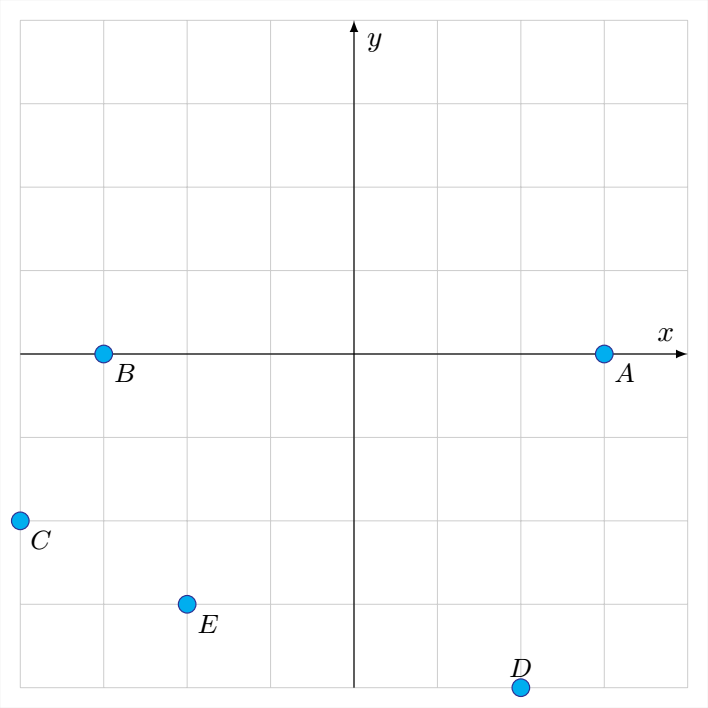
\includegraphics[width=\linewidth]{mex_0030.png}\\
				% Perímetro: \fillin[$40x-24y$][1in]
				% \part 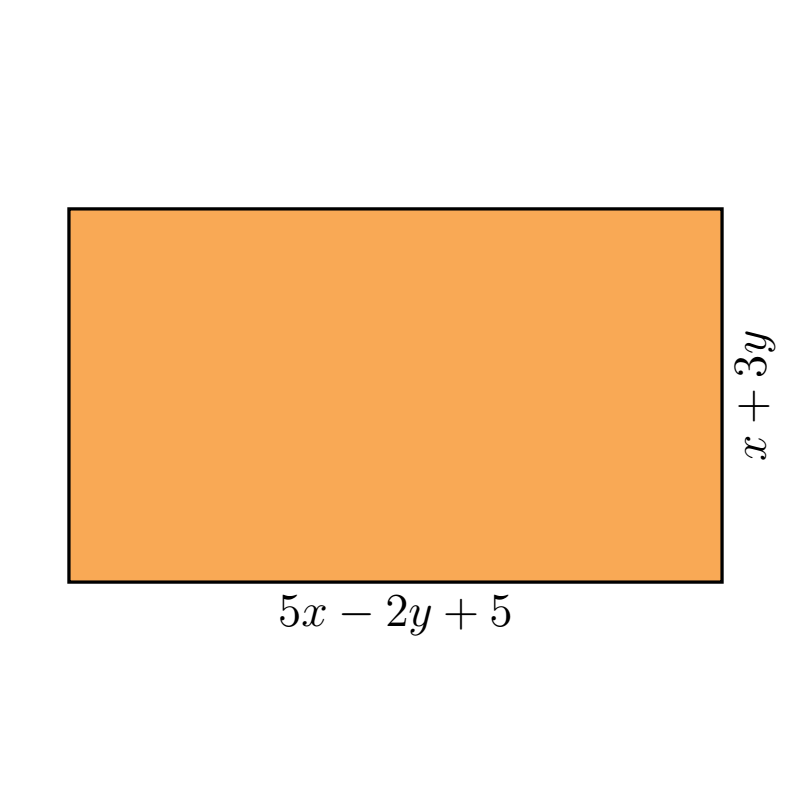
\includegraphics[width=1.2\linewidth]{mex_0031.png}\\
				% Perímetro: \fillin[$12x+2y+10$][1in]
				\part 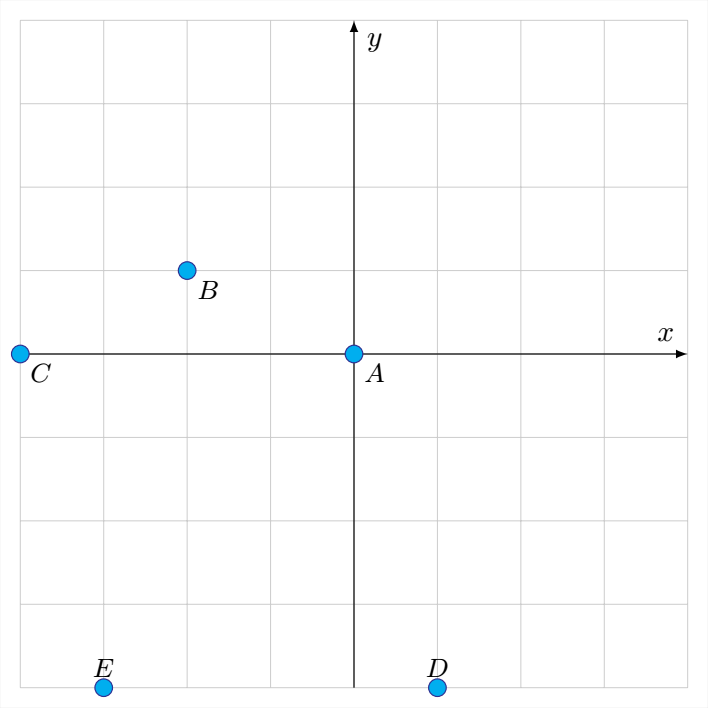
\includegraphics[width=.9\linewidth]{mex_0032.png}

				Perímetro: \fillin[$12a-18b-30$][0in]
				
				\part 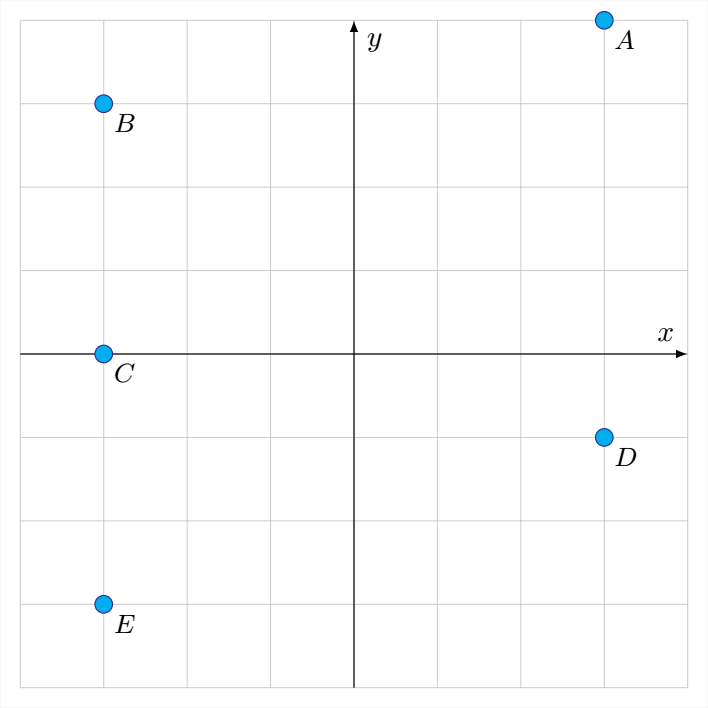
\includegraphics[width=.8\linewidth]{mex_0033.png}

				Perímetro: \fillin[$24x+48y-8$][0in]
				% \part 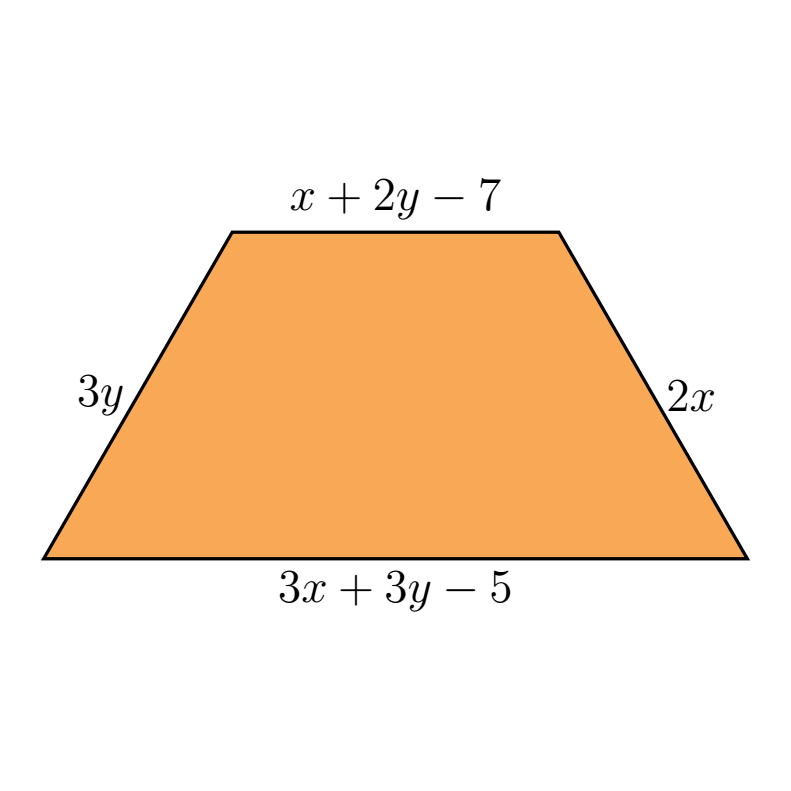
\includegraphics[width=\linewidth]{mex_0034.png}\\
				% Perímetro: \fillin[$6x+8y-12$][1in]
				\part 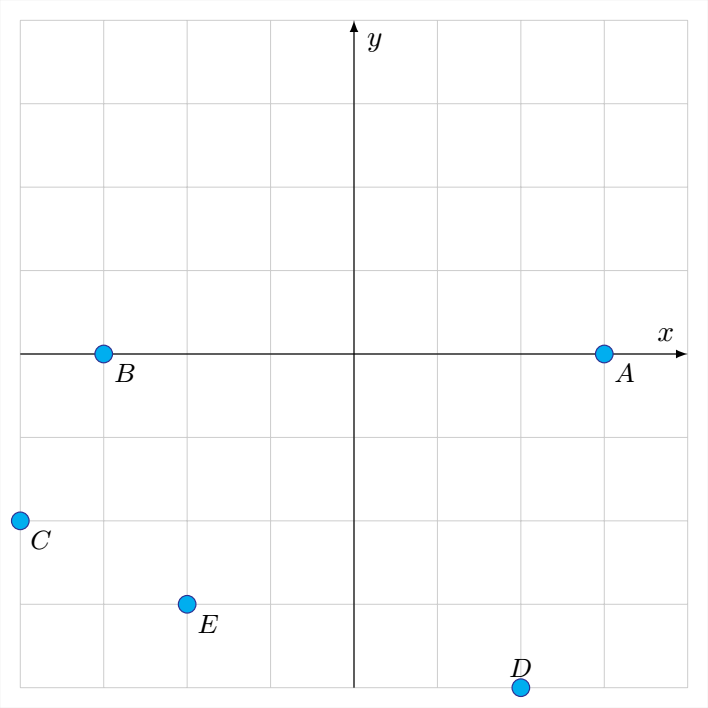
\includegraphics[width=.8\linewidth]{mex_0035.png}

				Perímetro: \fillin[$12x+4y-8$][0in]
			\end{parts}
		\end{multicols}
	}

	\newpage
	\section{Operaciones con monomios y polinomios}
	\subsection{Suma, resta y multiplicación de exponentes}

	\questionboxed[9]{Realiza las siguientes operaciones con exponentes:

		\begin{multicols}{3}
			\begin{parts}
				\subsection{Suma de exponentes}

				\part $(-3a^5)(8a^7)=$ \fillin[$-24a^{12}$][0in]

				\part $x^3yz^4 \cdot x^6z=$ \fillin[$x^9yz^5$][0in]

				\part $7x^2\cdot 3x^4 \cdot x^2=$ \fillin[$21x^8$][0in]

				\columnbreak%

				\subsection{Resta de exponentes}

				\part $\dfrac{x^{5}y^{4}z^{7}}{x^{2}y^{2}z^{6}}=$ \fillin[$x^3y^2z$][0in]

				\part $\dfrac{x^{4}yz}{x^{3}yz}=$ \fillin[$x$][0in]

				\part $\dfrac{81a^6b^{7}c^6}{9a^3b^{4}c^5}=$ \fillin[$a^3b^3c$][0in]

				\columnbreak%

				\subsection{Multiplicación de exponentes}

				\part $(ab^6c^3)^4=$ \fillin[$a^4b^{24}c^{12}$][0in]

				\part $\left(x^4 y^5\right)^2=$ \fillin[$x^8 y^{10}$][0in]

				\part $\left(a^2 b^4 c^{3} \right)^8=$ \fillin[$a^{16}b^{32}c^{24}$][0in]

			\end{parts}
		\end{multicols}
	}

	\subsection{Multiplicación y división de monomios y polinomios}

	\questionboxed[4]{Realiza la siguientes \textbf{multiplicaciones} de polinomios:

		\begin{multicols}{2}
			\begin{parts}
				\part $(x-3)(x^2-5x+4)=$ \fillin[$x^3-8x^2+19x-12$][0in] \\
				\part $(2a+3b)(4x+3y)=$ \fillin[$8ax+6ay+12bx+9by$][0in] \\
				\part $(x+1)(x+2)(x+3)=$ \fillin[$x^3+6x^2+11x+6$][0in] \\
				\part $(x+5)(2x^2+3x-7)=$ \fillin[$2x^3+13x^2+8x-35$][0in] \\
				\part $(x-1)(x+1)(x^2+1)=$ \fillin[$x^4-1$][0in] \\
				\part $(x+5)(x^2+2x-3)=$ \fillin[$x^3+7x^2+7x-15$][0in] \\
				\part $(x+3)(x-3)(x-2)=$ \fillin[$x^3-8x^2+21x-18$][0in] \\
				\part $(x+y)(x^2-xy+y^2)=$ \fillin[$x^3+y^3$][0in] \\
			\end{parts}
		\end{multicols}
	}

	\subsection{Áreas de figuras geométricas}

	\questionboxed[4]{Encuentra el \textbf{área} de las siguientes figuras:

		\begin{multicols}{4}
			\begin{parts}
				\part 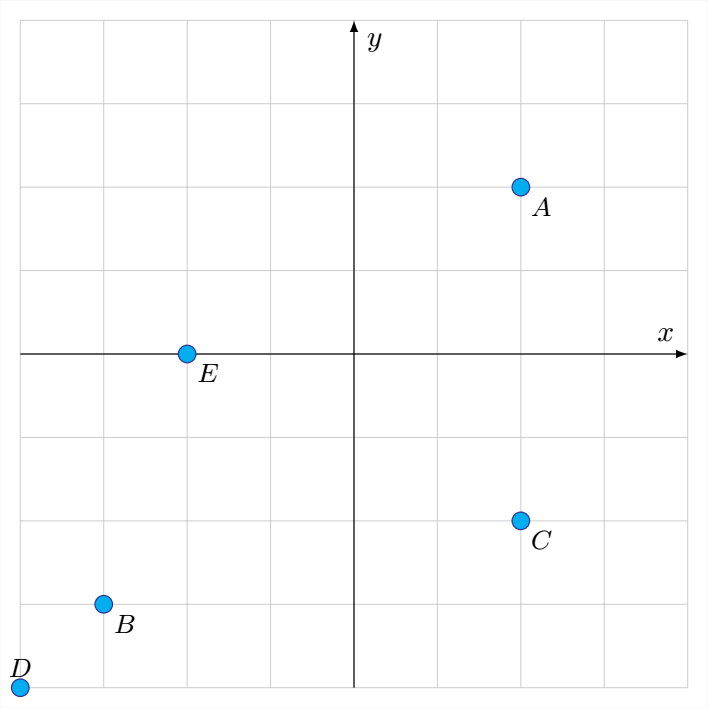
\includegraphics[width=.85\linewidth]{mex_0036.png}\\[0.5em]
				Área: \fillin[$x^2-6x+9$][0in]

				\part 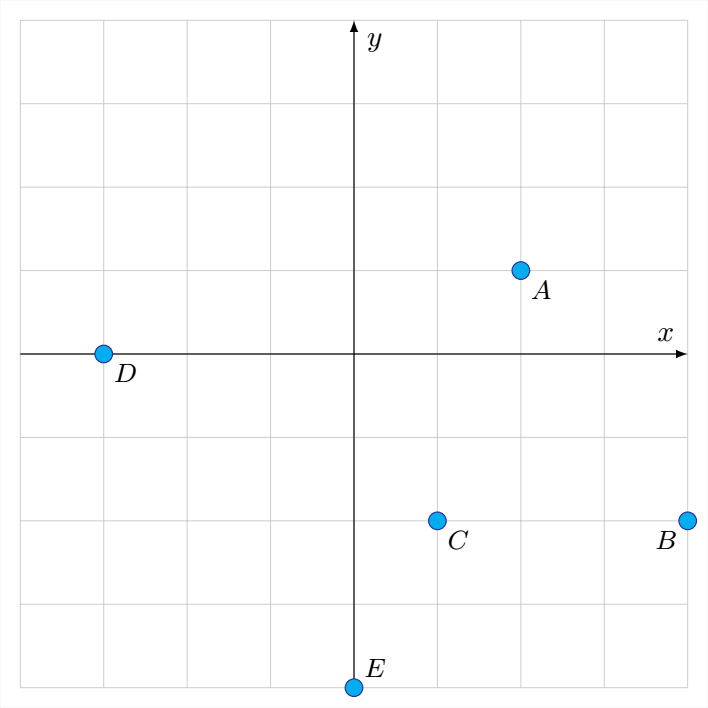
\includegraphics[width=1.2\linewidth]{mex_0037.png}\\[0.5em]
				Área: \fillin[$10x^2-50x$][0in]

				\part \includegraphics[width=1.2\linewidth]{mex_0038.png}\\[0.5em]
				Área: \fillin[$x^2+7x-30$][0in]

				% \part \includegraphics[width=\linewidth]{mex_0039.png}\\
				% Área: \fillin[$2x^2+4x$][1in]

				% \part \includegraphics[width=\linewidth]{mex_0040.png}\\
				% Área: \fillin[$2x^2+11x+14$][1in]

				\part \includegraphics[width=.85\linewidth]{mex_0041.png}\\[0.5em]
				Área: \fillin[$9x^2+12x+4$][0in]
			\end{parts}
		\end{multicols}
	}

	\newpage
	\section{Sistema de unidades}
	\subsection{Unidades de longitud y masa}

	\questionboxed[4]{Convierte las siguientes \textbf{unidades de longitud} y de \textbf{masa} como se te pide:

		\begin{multicols}{2}
			\begin{parts}
				% \part  3.8 kilómetros ($Km$) a metros ($m$).       \\ \fillin[$3.8\times 10 \times 10 \times 10=3800$][0in]
				\part  54 metros ($m$) a hectómetros ($Hm$).       \\ \fillin[$54\divisionsymbol 10 \divisionsymbol 10=0.54$][0in]
				\part  88 milímetros ($mm$) a centímetros ($cm$)   \\ \fillin[$88\divisionsymbol 10 =8.8$][0in]
				% \part  123 kilómetros ($Km$) a metros ($m$)		   \\ \fillin[$123\times 10 \times 10 \times 10=123000$][0in]
				\part  149 centímetros ($cm$) a decámetros ($Dm$). \\ \fillin[$149\divisionsymbol 10 \divisionsymbol 10 \divisionsymbol 10 =0.194$][0in]
				\part  6.5 gramos ($g$) a hectogramos ($Hg$).	   \\ \fillin[$6.5\divisionsymbol 10 \divisionsymbol 10=0.065$][0in]
				\part  8674 centigramos ($cg$) a gramos ($g$).     \\ \fillin[$8674\divisionsymbol 10 \divisionsymbol 10=86.74$][0in]
				\part  90.4 miligramos ($mg$) a centigramos ($cg$). \\ \fillin[$90.4\divisionsymbol 10 =9.04$][0in]
				\part  2.9 decagramos ($Dg$) a miligramos ($mg$).  \\ \fillin[$2.9\times 10 \times 10 \times 10\times 10=29000$][0in]
				\part  9.01 gramos ($g$) a miligramos ($mg$).      \\ \fillin[$9.01\times 10 \times 10 \times 10=9010$][0in]
			\end{parts}
		\end{multicols}
	}

	\subsection{Unidades de capacidad}

	\questionboxed[4]{Convierte las siguientes \textbf{unidades de capacidad} como se te pide:

		\begin{multicols}{2}
			\begin{parts}
				\part 27   hectolitros ($HL$) a centilitros ($cL$).       \\ \fillin[$27  \times 10 \times 10 \times 10\times 10=270000$][0in]
				\part 8    mililitros ($mL$) a centilitros ($cL$).        \\ \fillin[$8   \divisionsymbol 10 \divisionsymbol 10=0.08$][0in]
				\part 1094 mililitros ($mL$) a decilitros ($dL$).         \\ \fillin[$1094\divisionsymbol 10 \divisionsymbol 10=10.94$][0in]
				\part 702  mililitros ($mL$) a decalitros ($DL$).         \\ \fillin[$702 \divisionsymbol 10 \divisionsymbol 10\divisionsymbol 10 \divisionsymbol 10=0.0702$][0in]
				\part 1.9   litros ($L$) a mililitros ($mL$).             \\ \fillin[$1.9  \times 10 \times 10 \times 10=19000$][0in]
				% \part 8200 litros ($L$) a metros cúbicos ($m^3$).		  \\ \fillin[$8200\divisionsymbol 1000=8.2$][0in]
				 \part 4.8  decímetros cúbicos ($dm^3$) a litros ($L$).	  \\ \fillin[$4.8=4.8$][0in]
				\part 750  litros ($L$) a metros cúbicos ($m^3$).	 	  \\ \fillin[$750\divisionsymbol 1000=0.75$][0in]
				\part 567  milímetros cúbicos ($mm^3$) a litros ($L$).	  \\ \fillin[$567 \divisionsymbol 1000 \divisionsymbol 1000=0.000567$][0in]
				% \part 4100 litros ($L$) a metros cúbicos ($m^3$).		  \\ \fillin[$4100\divisionsymbol 1000=4.1$][0in]
			\end{parts}
		\end{multicols}
	}

	\subsection{Unidades de área y volumen}

	\questionboxed[10]{Convierte las siguientes \textbf{unidades de área} y \textbf{volumen} como se te pide:

		\begin{parts}
			\part  8.8 metros cúbicos ($m^3$) a milímetros cúbicos ($mm^3$) \\ \fillin[$8.8\times 1000 \times 1000 \times 1000=8800000000$][0in]
			\part  8 kilómetros cuadrados ($Km^2$) a metros cuadrados ($m^2$) \\ \fillin[$8\times 100 \times 100=80000$][0in]
			\part  88 metros cuadrados ($m^2$) a kilómetros cuadrados ($Km^2$) \\ \fillin[$88\divisionsymbol 100 \divisionsymbol 100\divisionsymbol 100=0.00088$][0in]
			\part  18 decámetros cúbicos ($Dm^3$) a centímetros cúbicos ($cm^3$)	\\ \fillin[$18\times 1000 \times 1000 \times 1000=18000000000$][0in]
			\part  801 milímetros cuadrados ($mm^2$) a decámetros cuadrados ($Dm^2$)	\\ \fillin[$801\divisionsymbol 100 \divisionsymbol 100\divisionsymbol 100 \divisionsymbol 100=0.000801$][0in]
		\end{parts}
	}
\end{questions}
\end{document}